\documentclass[11pt,a4paper,twoside,twocolumn]{article}

%--------------- Packages -------------------------------------------------
\usepackage{graphicx,parskip,times,amsfonts,amsmath}
\usepackage{jacobs-research-report}
\usepackage{eurosym}
\usepackage{natbib}
\usepackage{a4,a4wide}
\usepackage[latin1]{inputenc}
\usepackage[english]{babel}
\usepackage{amssymb,amsmath,amsfonts}
\usepackage{bibunits}
\usepackage{longtable}
\usepackage{bpchem}
%---------------------PDF-definitions--------------------------------------
\usepackage[pdftex,           %%% hyper-references for pdflatex
  hypertexnames=false,%       %%% needed for correct links to figures
  breaklinks=true,%           %%% break links if exceeding a single line
  colorlinks=true,%           %%% to underline links instead of boxing
  urlcolor=blue]{hyperref}    %%% blue instead of cyan URLS
%--------------------end-of-PDF-definitions-------------------------------
\usepackage{makeidx}
\makeindex

%--------------------User Definitions----------------------------------------
\hyphenation{Schlei-cher} \hyphenation{geo-me-try}
\newcommand{\C}{\mathbb{C}}
\newcommand{\R}{\mathbb{R}}
\usepackage{latexsym}
\newcommand{\bbbr}{\mathbb{R}}
\newcommand{\bbbn}{\mathbb {N}}
\newcommand{\bbbc}{\mathbb {C}}
\newcommand{\mycaption}[1]{\caption{#1}}
\renewcommand*{\cleardoublepage}{\clearpage\if@twoside \ifodd\c@page\else
    \hbox{}
    \if!\blankpagetext!\else
    \vfil \begin{center} \setlength{\fboxsep}{3mm}%
    \framebox{\blankpagetext}
    \end{center}\vfil\vfil \fi
    \newpage\if@twocolumn\hbox{}\newpage\fi\fi\fi}
\newcommand*{\resetpages}{\cleardoublepage\pagenumbering{arabic}}
\raggedbottom \pagenumbering{Roman}
\newenvironment{myitemize}{\begin{list}{-}{\labelwidth=0.2cm \leftmargin0.4cm
\labelsep0.2cm \rightmargin0cm \parsep0.5ex plus0.2ex minus0.1ex
\itemsep0ex
 plus0.2ex}}{\end{list}}

% new line after paragraph heading
\makeatletter
\newcommand\myparagraph{%
\@startsection{paragraph}{4}{\z@}%
{-3.25ex \@plus1ex \@minus.2ex}%
{.15ex \@plus.1ex \@minus.1ex}%
{\normalfont\normalsize\bfseries}}
\makeatother

\setlength{\parskip}{0pt plus 1pt}

%---------------------- Document ------------------------------------------------
\begin{document}
\def\Hchapter{\paragraph}
\def\bpchem{\BPChem}
%---------------- Path for images and pictures -------------------------------------
\graphicspath{{./MathTheoPhys/}{./Nano/}{./LifeSciences/}{./ESS/}{./EECS/}}


%----------------Title -------------------------------------------------------------
\title     {School of Engineering and Science \\
            Research Report 2007/2008} \shorttitle{RP 2007/2008}
\author    {Anke Allner}
\date      {2009 January}
\masterfile{SES--RR--2007/2008}
\issue     {0}
\revision {1}
\version {2}{0}{05.01.09}{Test}
%-----------------------------------------------------------------------------------
\renewcommand{\refname}{\medbreak Publications\vadjust{\nobreak}}
\renewcommand{\bibname}{\medbreak Publications\vadjust{\nobreak}}
%-----------Table of Contents one column -------------------------------------------
\onecolumn
\shorttitle{Table of Contents} \tableofcontents \resetpages

%----------- Switch to two columns ----------------------------------------------------
\twocolumn

%------------ Into Dean ---------------------------------------------------------------
\shorttitle{Introduction}
\section{Introduction}

With the outstanding financial investment of the Jacobs Foundation
in the Jacobs University on October 31, 2006 the future perspective
of the University and in particular the School of Engineering and
Science is on steady and forseeable grounds. This, and the advent of
the new president Professor Dr. Dr. h.c. mult. Joachim Treusch, who
formally took office by July 1, 2006, eventually resulted in a
reformulation of the key mission and the main research objectives of
the university. The main scientific activities of the School can be
considered to be perfectly consistent with the new objectives.

\subsection{The Mission}

The Jacobs University Bremen has been designed and developed as an
international research university using the anglo-saxon template,
and incorporating the European Bologna Process into its teaching
model. The main mission is to academically educate bright young
people, irrespective of their nationality, religion, sex, race and
financial conditions, in order to prepare them for future leading
roles in our globalized world. Thus, the University is designed to
provide significant contributions towards a peaceful, and
sustainable development of mankind. As a campus university where
students from more than 80 nations live and learn together in
colleges, intercultural understanding and collaboration in daily
life is trained as a byproduct of the university education.

\null
 Research and teaching are pursued on the same level and take
into account the requirements of practical life in enterprises and
industry. Interdiciplinarity constitutes the key concept. Research
at the Jacobs University Bremen aims at delivering key contributions
towards the main challenges of mankind, namely \\

\begin{myitemize}
\item   energy and materials,
\item  water and food,
\item   health,
\item "Bildung" and communication,
\item peace and conflict management.
\end{myitemize}


\null
 The School of Engineering and Science contributes with its
activities mainly towards the former three of these, although its
strong electrical engineering faculty addresses technological issues
that are closely related to the latter two.

The scientific objectives of Jacobs University concentrate in five
broad areas, namely \\

\begin{myitemize}
\item bio-geo-marine resources - from molecules towards technologies
\item  modelling of complex systems - computer simulation, visualisation, networks and management
\item changing societies, cultures, and institutions -  aspects of globalisation
\item   Asia and Europe - historical,
psychological and cultural perspectives
\item productive adult development \item "Bildung" and work
\end{myitemize}


\null
 The five research fields of the School of Engineering and
Science that have been emerging during the founding years contribute
towards the first two of these: Projects within "Information and
Communication Technologies" are directly related to the second
research area. Topics addressed by our "Life Sciences" and
"Geosciences and Astrophysics"  contribute to the first as well as
to the second area. "Nanoscience and Material Research" and
"Mathematics and Theoretical Physics" establish the scientific
backbones of the above. These provide important scientific tools and
the key methods for successfully tackling questions at the
interfaces between the conventional disciplines.

\null
The latter, namely science across disciplinary boarders is
indeed the outstanding - if not the main - trademark of research and
development,  and teaching at the  School of Engineering and
Science.


\subsection{Factual Development During the Founding Period}

\subsubsection{Students}
During the course of the past founding years, the School of
Engineering and Science has been showing remarkable growth, in
quantity as well as in quality. The number of undergraduate
students, starting in 2001 with 67 has now reached its preliminary
saturation at 381 students (Fig.~\ref{fig:students}). Basically this
is dictated by the number of college places and the fact that
according to planning 2/3 of the total number of students can be
admitted to programs of the School. There are now 12 undergraduate
programs of which 10 are formally accredited.


In 2004, for the first time a significant number (48) of graduate
students were admitted to the graduate programs of the School. Since
then, the number of graduate students has been growing to an
impressive total of 223 out of which 142 are PHD-students
(Fig.~\ref{fig:students}). By now, the school has successfully
established 7 graduate programs on the master's level.

\begin{figure}[ht]
  \begin{center}
   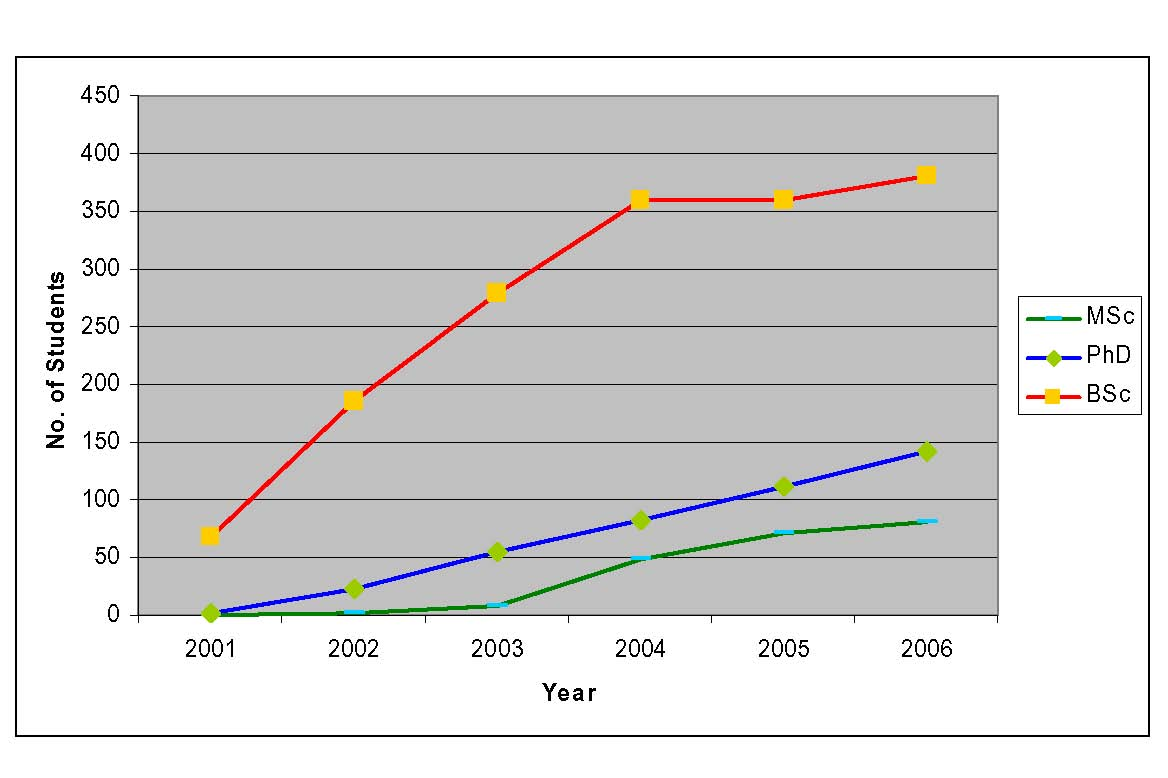
\includegraphics[width=\hsize]{Students.jpg}
   \end{center}
\caption{Temporal Development of Number of Students in the School of
Engineering and Science \label{fig:students}}
\end{figure}

\label{students}

\subsubsection{Publications}

During the founding period, the scientific output of the School,
measured in terms of the number of publications, has been growing
from initially 144 to 389 in 2006, after an intermediate decrease in
2004 which can be understood by having in mind that 2004 has been
the year during which the main research laboratories have been
planned and constructed (Fig.~\ref{fig:publications}). The last of
the laboratories (the EON laboratory) has been finished in 2005.

\begin{figure}[ht]
  \begin{center}
   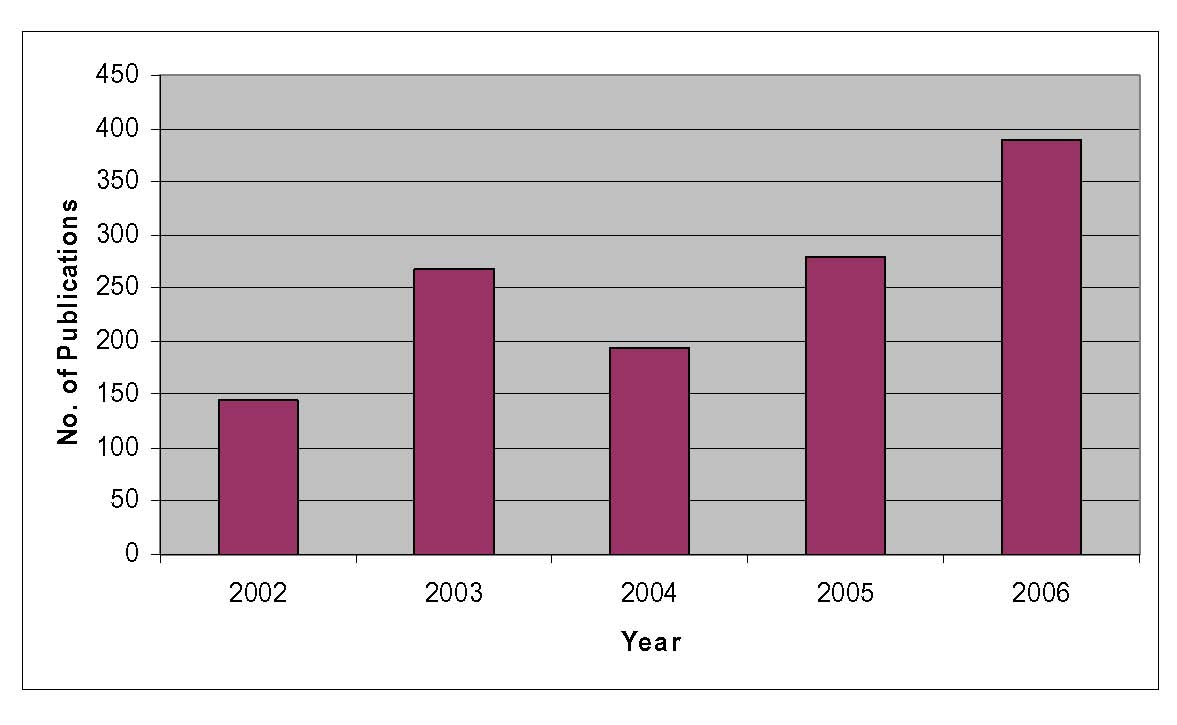
\includegraphics[width=\hsize]{Publications.jpg}
   \end{center}
 \caption{Number of Peer-reviewed Articles, Conference Proceedings, Articles in Encycl./Handbooks,
 Monographs/Books, Editor-ship, and Contribution in Ed. Volumes
 \label{fig:publications}}
\end{figure}


\subsubsection{Grants}
The development of third party funding is summarized in Figures
\ref{fig:grants1}, \ref{fig:grants2}. Revenues from Research grants
have reached a total of more than 4.000.000 EURO in 2006 which
implies an average revenue per professor of 82.000 EURO.

\begin{figure}[ht]
  \begin{center}
   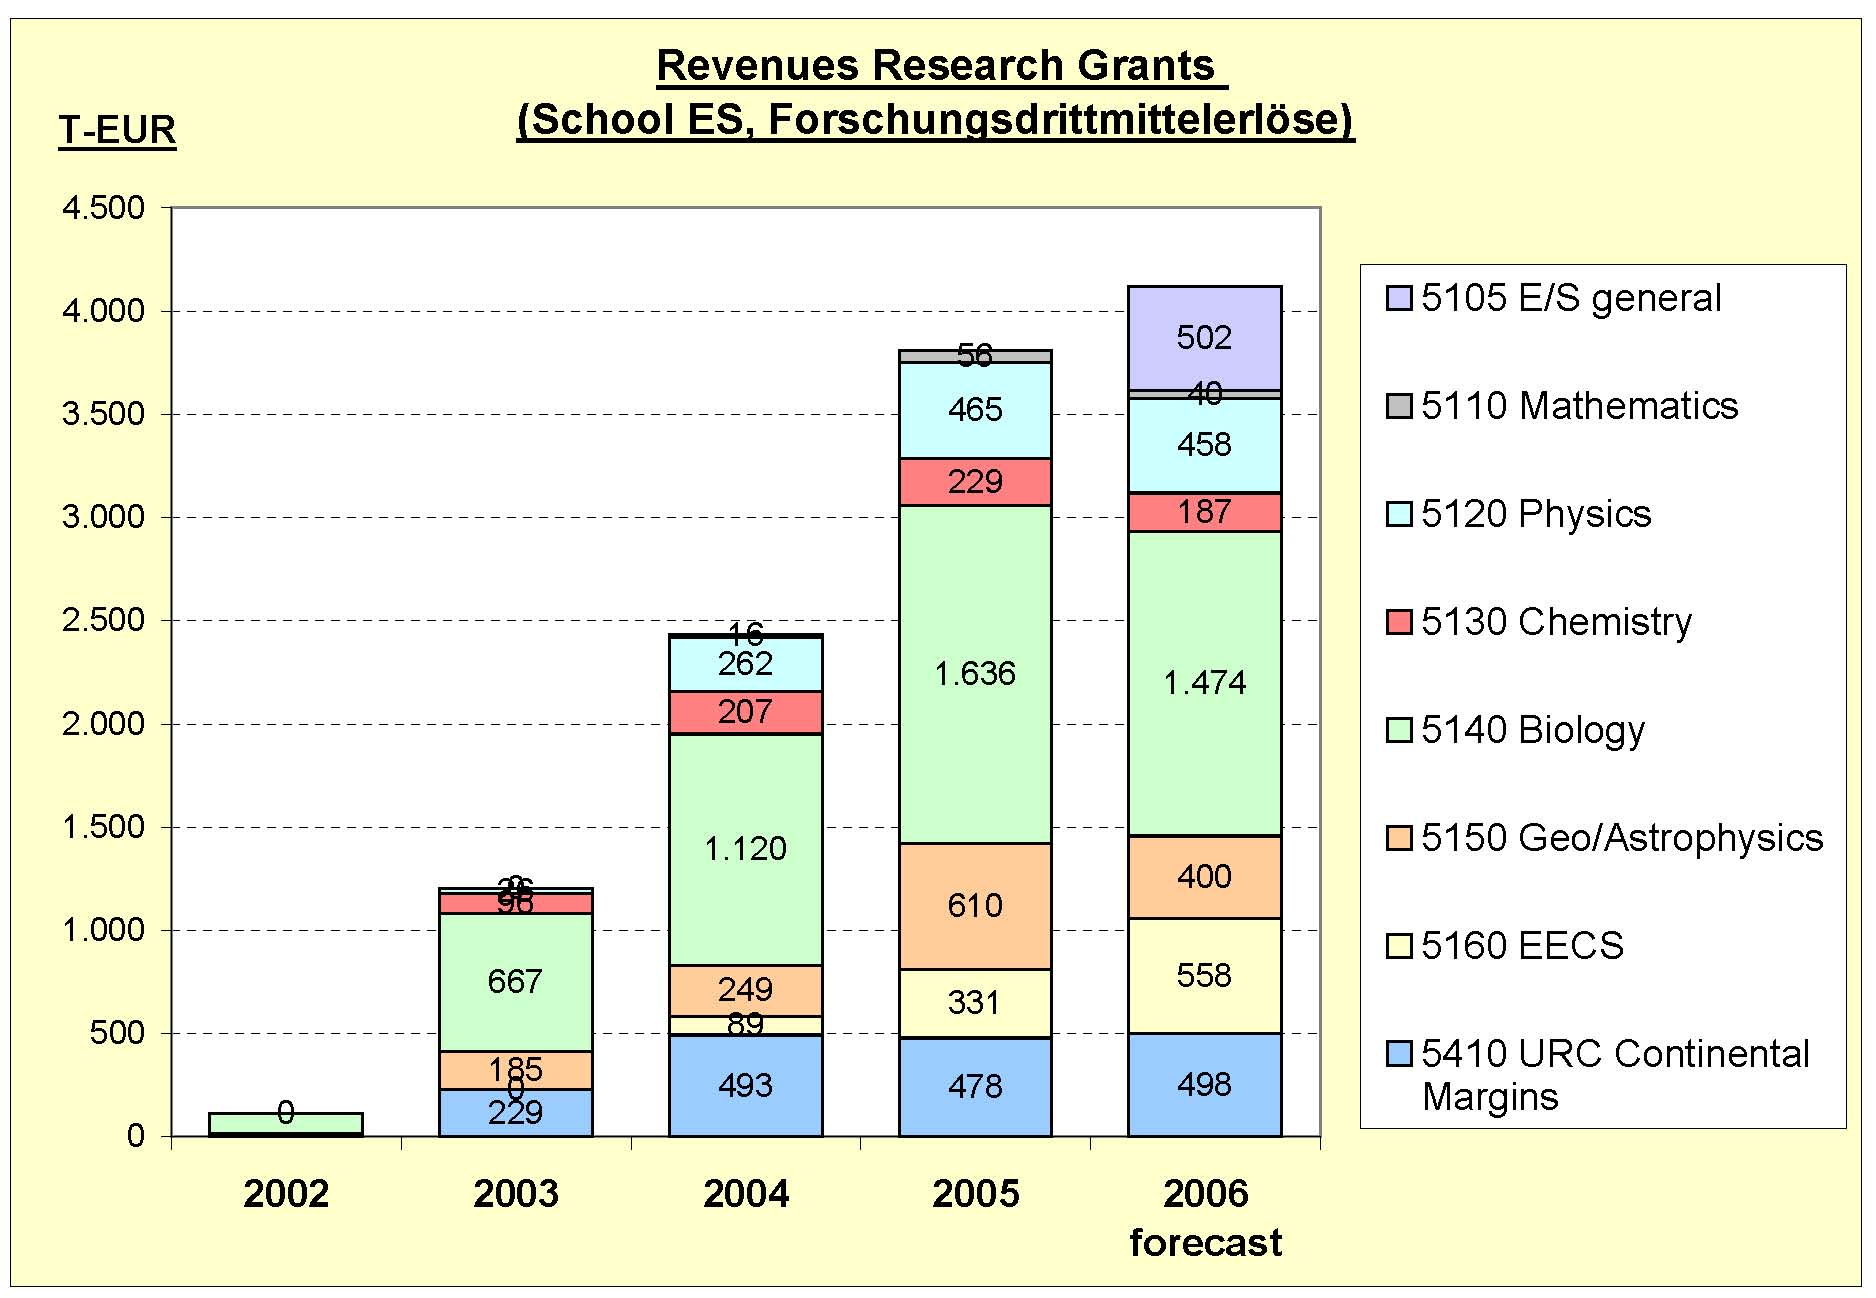
\includegraphics[width=\hsize]{SchoolESGrants-Charts1.jpg}

   \end{center}
 \caption{Research Grants  Revenue
 \label{fig:grants1}}
\end{figure}

\begin{figure}[ht]
  \begin{center}
   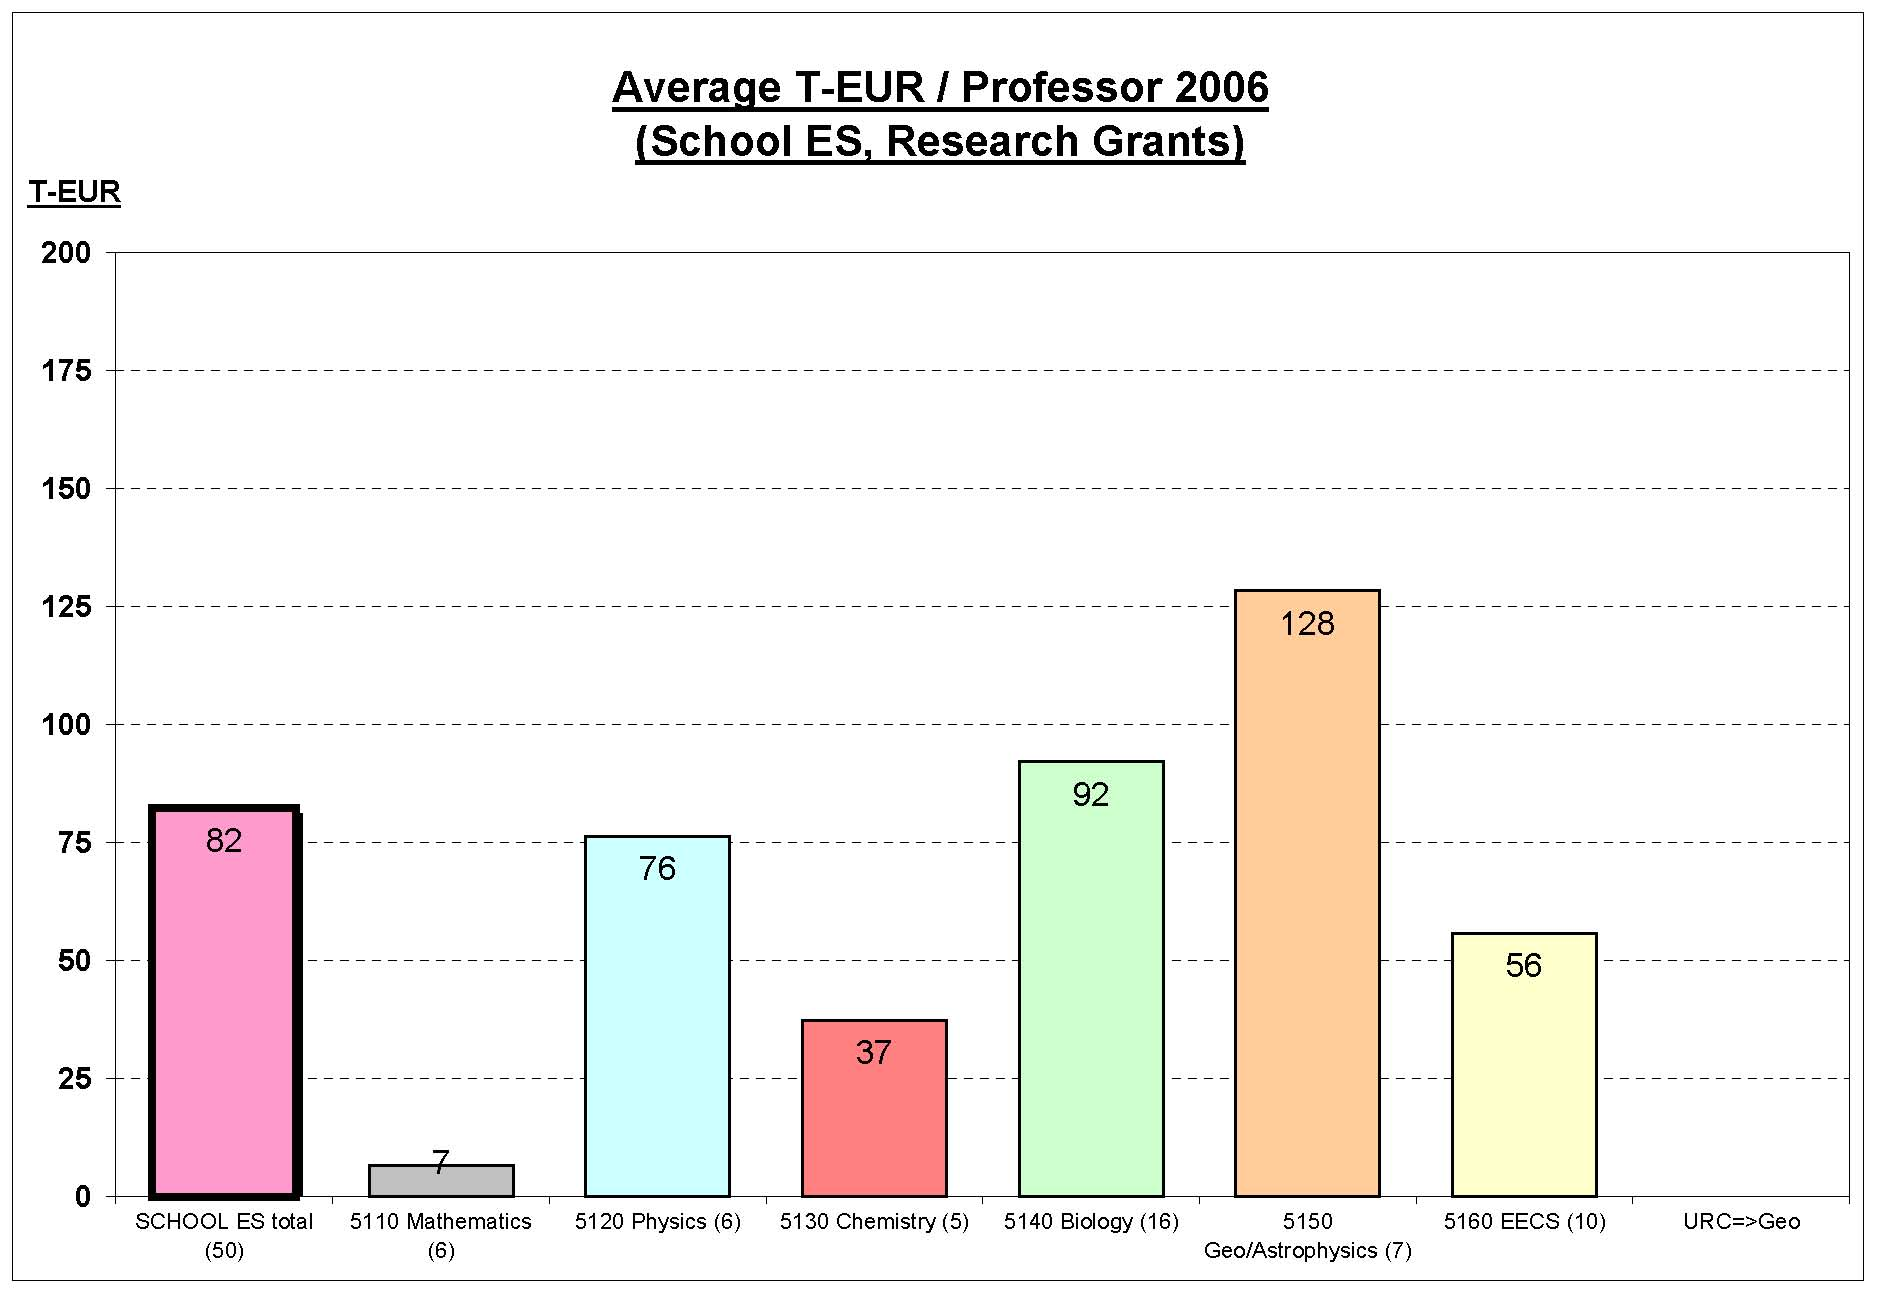
\includegraphics[width=\hsize]{SchoolESGrants-Charts2.jpg}
   \end{center}
 \caption{Research Grants Average T-EUR/Professor
 \label{fig:grants2}}
\end{figure}

\subsection{Personnel 2006} Presently, the school comprises in
total 64 professors out which 4 are adjunct professors, located at
the Alfred-Wegner-Institut in Bremerhaven and the Max-Planck-Insitut
f�r Marine Mikrobiologie in Bremen. Two distinguished professors and
6 university lecturers complete the faculty. In addition, 70
research associates, 5 research assistants, 26 technicians, 1
director and 7 assistants belong to the staff. In 2006, several new
faculty members have been hired.

\begin{myitemize}
 \item   Dr. Ulrich Kleinkath\"ofer, Associate Professor of
Theoretical Physics \item  Jon Wallace, PhD, Assistant Professor of
Electrical Engineering \item  Dr. Lars Linsen,  Associate Professor
of Computational Science and Computer Science \item   Dr. Bendick
Malehko, University Lecturer in Computer Science.
\end{myitemize}

In Mathematics, the visiting professors Prof. G. Litvinov and Prof.
Vladimir Tikhomirov, and Dr. Marc Comerford (research instructor)
left. They are replaced by \begin{myitemize} \item  Dr. Stefan Baier
(Visiting Lecturer for Mathematics) \item Kaivan Mallahi-Karai (PhD,
Visiting Lecturer for Mathematics) \item Dr. Alexei Belov (Visiting
Professor for Mathematics).
\end{myitemize}

The following members of the faculty have been promoted during 2006.
\begin{myitemize}
\item  Dr. Klaudia Brix from Associate to Full Professor
\item Dr. Albert Jeltsch from Associate to Full Professor
\item   Dr. Laurenz Thomsen from Associate to Full Professor
\item Marcus Br\"uggen Assistant to Associate
\item Claus C. Hilgetag, PhD from Assistant to Associate
\item Dr. Ulrich Schwaneberg from Assistant to Associate
\end{myitemize}

\null
Dr. Stefano Carpin, Assistant Professor of Computer Science,
has accepted an offer of an Assistant Professorship at University of
California, Merced, USA, starting on January 1, 2007.

\subsection{International Center for Transdisciplinary Science}
 The "International Center for Transdisciplinary Studies"
has been founded and started to operate. The center invites
internationally highly ranked scientists as fellows for periods of
several weeks, mostly during the summer break. The visiting
scientists are generally expected to participate in ongoing
scientific activities. In 2006, 46 scientists have been
participating, among them 39 from foreign countries:

\null Professor Dr. Roland Benz,   Universit\"at W\"urzburg, Germany
\\
Professor Dr.~Jan Bergstra,  University of Amsterdam, The Netherlands\\
Dr.~Andrey Bessonov, University of Sankt Petersburg, Russia\\
Dr.~S.M. Bezrukov,  National Institute of Health, Bethesda, USA\\
Dr. Georges Bouzerar,   Laboratoire Louis Nel, Grenoble, France\\
Dr. Henk Bruin  University of Surrey, United Kingdom\\
Professor Dr.~Mark Burgess,  University College Oslo, Norway\\
Professor Dr.~Val\'erie Cabuil,     Universit\'e Pierre et Marie
Curie, Paris, France\\
Dr.~Fabio Cavaliere, Universit\'a di Genova, Italy, Professor
Dr.~Shengbo Chen,      Institute of Geography and Natural
Resources, Beijing, China\\
Elizabeth Dan-Cohen,     University of California, Berkeley, USA\\
Professor Dr.~Gero Decher,      Institut Charles Sadron, Strasbourg,
France\\
Dr.~Martin Evans,        University of Edinburgh, United Kingdom\\
Dr.~Tom Fisher,      University of Cambridge, United Kingdom\\
Dr.~Claus F\"utterer,       Institut Curie, Paris, France\\
Professor Dr.~Mariano Grasselli,     Universidad Nacional de
Quilmes,
Argentina\\
Dr.~Giovanni Indiveri,       University of Lecce, Italy\\
Professor Dr.~Dieter J\"ager,      Emory University Atlanta, USA\\
Professor Dr.~Larry S. Liebovich,        Florida Atlantic
University,
USA\\
Professor Liviu Movileanu,      Syrakuse University, USA\\
Dr.~Sergei Nechaeev     CNRS Orsay, France\\
Professor Dr.~Catherine O'Neill,     Columbia University, USA\\
Dr.~Marieke Postma,     NIKHEF, Amsterdam, The Netherlands\\
Dr.~Enrico Ramirez-Ruiz,     Institute of Advanced Studies,
Princeton, USA\\
Professor Dr.~Helmut Ringsdorf,      Universit\"at Mainz, Germany\\
Dr.~Karin R\"omisch,       University of Cambridge, United Kingdom\\
Lucile Sassatelli,       ENSEA-ETIS, Cergy-Pontoise, France\\
Professor Dr.~J\"urgen Schnack,        Universit\"at Osnabr\"uck,
Germany\\
Professor Dr.~Gerhard Schwarz,       Biozentrum Basel, Switzerland\\
Professor Dr.~Vera Serganova,        University of California,
Berkeley, USA\\
Professor Dr.~Nobuo Shimamoto,      National Institute of Genetics,
Mishima, Japan\\
Professor Dr.~Canan Tari,        Izmir Institute of Technology,
Turkey\\
Professor Dr.~Alexander Tikhomirov,  Yaroslavl State Pedagogical
University, Russia\\
Dr.~Andrew Travers,      Medical Research Council, Cambridge, United
Kingdom\\
Dr.~Martin Weigt,        ISI Foundation, Torino, Italy\\
Professor Dr.~James Whisstock,      Monash University, Victoria,
Australia\\
Dr.~Wojtek Zakrzewski,   University of Durham, United Kingdom\\
Dr.~Michael Zaks,    Humboldt-Universit\"at Berlin, Germany\\
Professor Dr.~Gregg Zuckerman,   Yale University, USA.

\subsection{Workshops and Summer Schools 2006}

During the year, several international research workshops have been
organized on the campus by members of the faculty.

\begin{myitemize}
\item
From October 19-22, 2006 the International Workshop on Astrobiology
took place at IUB, organized by Professor Michael Bau.  Focus of the
workshop were Banded Iron Formations (BIFs), that developed between
two and four billion years ago in the precambrian era.  The workshop
aimed at providing an overview on current ideas on the formation and
preservation of Precambrian BIF, on the use of BIF as proxies for
Precambrian seawater, on differences between Early Precambrian BIF
and younger ironstones and hydrogenetic Fe(-Mn) precipitates, and on
experimental set-ups to simulate BIF-related processes in Early
Precambrian environments.

\item
A workshop for young scientists is offered biannually by the DFG
Schwerpunktprogramm SPP1170 (priority program) ''Directed Evolution
to Optimize and Understand Molecular Biocatalysts''. This year's
workshop  took place from July 30 until August 1 on the IUB campus,
organized by Professor Ulrich Schwaneberg. 70 scientists from the 17
DFG institutions participate in the program. They presented and
discussed the research and its influence on applications with
representatives from companies.


\item
From July 28 until August 5, a Summer School for students and
postdocs  took place. Focus of the more than 50 lectures and
workshops has been on recent research perspectives in biosensing and
its application. 70 participants from 14 Nations met on IUB campus.
This summer school  covered applications of membrane channels in
molecular biology and biotechnology. In addition, it informed on the
underlying physics and will present recent advances in microfluidics
and nanoelectronics. The fourth IUB Summer School has been organized
by Dr. Mathias Winterhalter, Professor of Biophysics at IUB. The
Summer School offered students and postdocs the opportunity to
advance their understanding of biosensing, present their research
and build networks.


\item In June 2006, the 10th International RoboCup has been organized
in Bremen. More than 400 teams and 2500 participants from 36
countries participated and competed in three main categories: the
robot soccer competition, the robot rescue competition (coordinated
by Prof. A. Birk), and the RoboCupJunior for educational purposes.
On June 18, the finals of the Robot Rescue League took place in the
Congress Center Bremen. IUB teams participated in both competitions
the ''Rescue Robot League�� and the ''Virtual Robot Competition��.
The team led by Andreas Birk, Professor of Electrical Engineering
and Computer Science, reached the finals of the Robot League and won
the Innovation Award, a student team led by Stefano Carpin,
Professor of Computer Science came in second place in the Virtual
Robot Competition.

\item
From the 16th to 20th of January, IUB  hosted the international
"HERMES Graduate Training and Job Fair". More than 30 Master's and
PhD students working at HERMES partner institutions all over Europe
participated. The fair offered students and Postdocs the opportunity
to advance their understanding in aspects of marine science outside
their own fields and to present and discuss their own research (Jan
10, 2006). The HERMES (Hotspot Ecosystem Research on the Margins of
European Seas) Program, funded by the European Commission, was begun
to gain better understanding of life in depths of between 200 and
2000 meters and deeper.

\end{myitemize}


\subsection{Research Highlights}

Researchers of the School of Engineering and Science have been
contributing towards the international scientific progress with
several important discoveries that have been published in the most
prestigious international journals.

\begin{myitemize}
\item
Albert Jeltsch, IUB Professor of Biochemistry, and his co-workers
from IUB, the Institute of Biochemistry of the University of
Giessen, and the Medical Research Council of Cambridge University
(UK) for the first time successfully used genetically engineered
proteins to deactivate Herpes viruses in human cell lines. The study
is published in the November 2006 issue of Nucleic Acids Research

\item
Stefan Tautz, IUB Professor of Physics, and his group for the first
time managed to detect a much larger delocalization of electrons in
an organic monolayer semiconductor deposited on a metallic substrate
than ever detected in an insulated organic semiconductor. The
results, which were published in Nature 444, p. 350 - 353, on
November 16, 2006, allow insights into basic mechanisms of electron
transport within organic materials and their interfaces with
metallic surfaces. Moreover, the results may be of relevance for the
development of new hybrid materials with interesting new electronic
properties regarding future application.



\item
On the 68th cruise of the German research vessel METEOR an
international team of scientists under the lead of Andrea
Koschinsky, Professor of Geosciences at IUB, registered 407
$^{\circ}$ C at a hydrothermal vent as the highest temperature on
record measured at the ocean bottom (May 22, 2006).  Using a special
temperature sensor operated by a deep-sea robot the scientists
registered the record temperature in 3000m water depth at a
so-called ''black smoker'', a hydrothermal deep-sea vent with a
characteristic particle plume in the discharge water. Moreover, the
boiling fluids emitted by the vent were filmed. The super-hot vent
was discovered at 5 $^{\circ}$ S at the Mid-Atlantic Ridge, where
the African and the South American continental plates drift apart 4
cm per year, causing increased volcanic activity. Normally the
temperature of the circulating seawater cooling the volcanoes
emerging in this area does not exceed a maximum of about 350
$^{\circ}$ C when welling out of the sea floor. Maximum deep-sea
water temperatures up to 402 $^{\circ}$C so far have only been
observed in the Pacific.




\item
Stephan Rosswog, Professor of Astrophysics at IUB, and Daniel Price,
Postdoc at the University of Exeter, for the first time were able to
demonstrate in supercomputer simulation of a neutron star merger
that a collision of these super dense cosmic objects create magnetic
fields a quadrillion (10$^{15}$) times stronger than the magnetic
field of the earth. The simulation results are published in the
current online express issue of Science ("Producing ultra-strong
magnetic fields in magnetized neutron star mergers", 30 MARCH 2006).

\item
Claus Hilgetag, Professor of Neuroscience at IUB, and his colleague
Helen Barbas, Professor of Health Sciences at Boston University,
found new answers to one of the oldest questions in neuroscience:
How do the characteristic folds of the primate brain cortex form?
The results of an extensive analysis of neuroanatomic data are
published as the cover story in the latest issue of PLoS
Computational Biology ("Role of Mechanical Factors in the Morphology
of the Primate Cerebral Cortex", Volume 2, Issue 3, MARCH 2006,
www.ploscompbiol.org).  By analyzing quantitative data collected in
the lab of Helen Barbas over a period of two decades, Claus Hilgetag
for the first time was able to provide empirical evidence for the
hypothesis that the characteristic folds of the primate brain are
mainly formed by mechanical forces of fiber tension.


\end{myitemize}


\subsection{Noteworthy}
\begin{myitemize}
\item
On November 15, 2006, the association ''Unifreunde e. V.�� awarded
the Ernst A. C. Lange Prize for the joint research project ''New
display technology for mobile applications�� of IUB and University
of Bremen. The award, which is endowed with 5000 euros prize money,
acknowledges innovative co-operational research between scientists
of the two Bremen universities in the fields of Mathematics, Natural
and Technical Sciences. The two laureates 2006 are the two Bremen
scientists Dietmar Knipp, Professor of Electrical Engineering at
IUB, and Wolfgang Benecke, Professor of Physics, Electronics and
Information Technology at University of Bremen. The aim of their
joint research project is the development of a new type of
projection display for mobile application such as laptop computers,
mobile phones, and digital cameras.


\item Researchers from all over Germany were taking part in the Science
Festival "Highlights of Physics" from 6-10 November 2006 in Bremen.
Under the motto of "WaveWorlds" scientists gave an introduction into
wave phenomena in water, light and sound through series of talks,
live experiments and science shows.  IUB was involved in the
organization and preparation of this event. Faculty and staff
contributed in particular to the big opening show, the exhibition,
and the physics competition for pupils.

\item
In October the research network International Research Consortium on
Continental Margins (IRCCM) under IUB's lead started a new research
project on biomonitoring of cold water coral reefs in the vicinity
of oil exploration sites. The aim of the 1.2 million euro project
financed by the Norwegian company Statoil is to develop new
monitoring and ecosystem modelling approaches for risk assessment in
the off-shore industry.  Research site is the Tisler cold water
coral reef in the Skagerrak, which was placed under environmental
protection by the Norwegian government in 2003. As part of the EU
HERMES project (Hotspot Ecosystem Research on the Margins of
European Seas) it is managed by HERMES partner Tj\"arn\"o Marine
Biological Laboratory (TMBL) and will host IUB's second deep-sea
online observatory.


\item
On April 23, 2006, IUB's RoboCup team managed another international
tournament victory at the US Open Robot Rescue League in Atlanta,
prevailing against the other competing institutions only two weeks
after their success at the Dutch Open in Eindhoven (Apr 25,2006).
The ten contesting teams in Atlanta included such renowned
institutions as the Georgia Institute of Technology and Carnegie
Mellon University, which demonstrated with their impressive
investments into their teams the importance of research on search
and rescue robots in the US. Georgia Tech had two teams within the
competition, one of them using the best mobile research platform
that is currently available on the market. A team from Carnegie
Mellon University had even six robots running including a high-end
commercial platform for search and rescue missions.

\item
Informatics Year is being organised in conjunction with the Science
in Dialogue initiative and the Gesellschaft f�r Informatik (GI) as
well as with numerous partners in the fields of science, industry
and culture. The idea behind this Science Year was to familiarise a
broader public with the contents, processes and practical
applications of science and to do so in an informative, exciting and
entertaining way. IUB was involved in exhibitions, the Symposium on
Artificial Intelligence and various other activities.

\end{myitemize}
\ \ \\
\ \ \\

Bremen, January 2007


\begin{figure}[ht]
     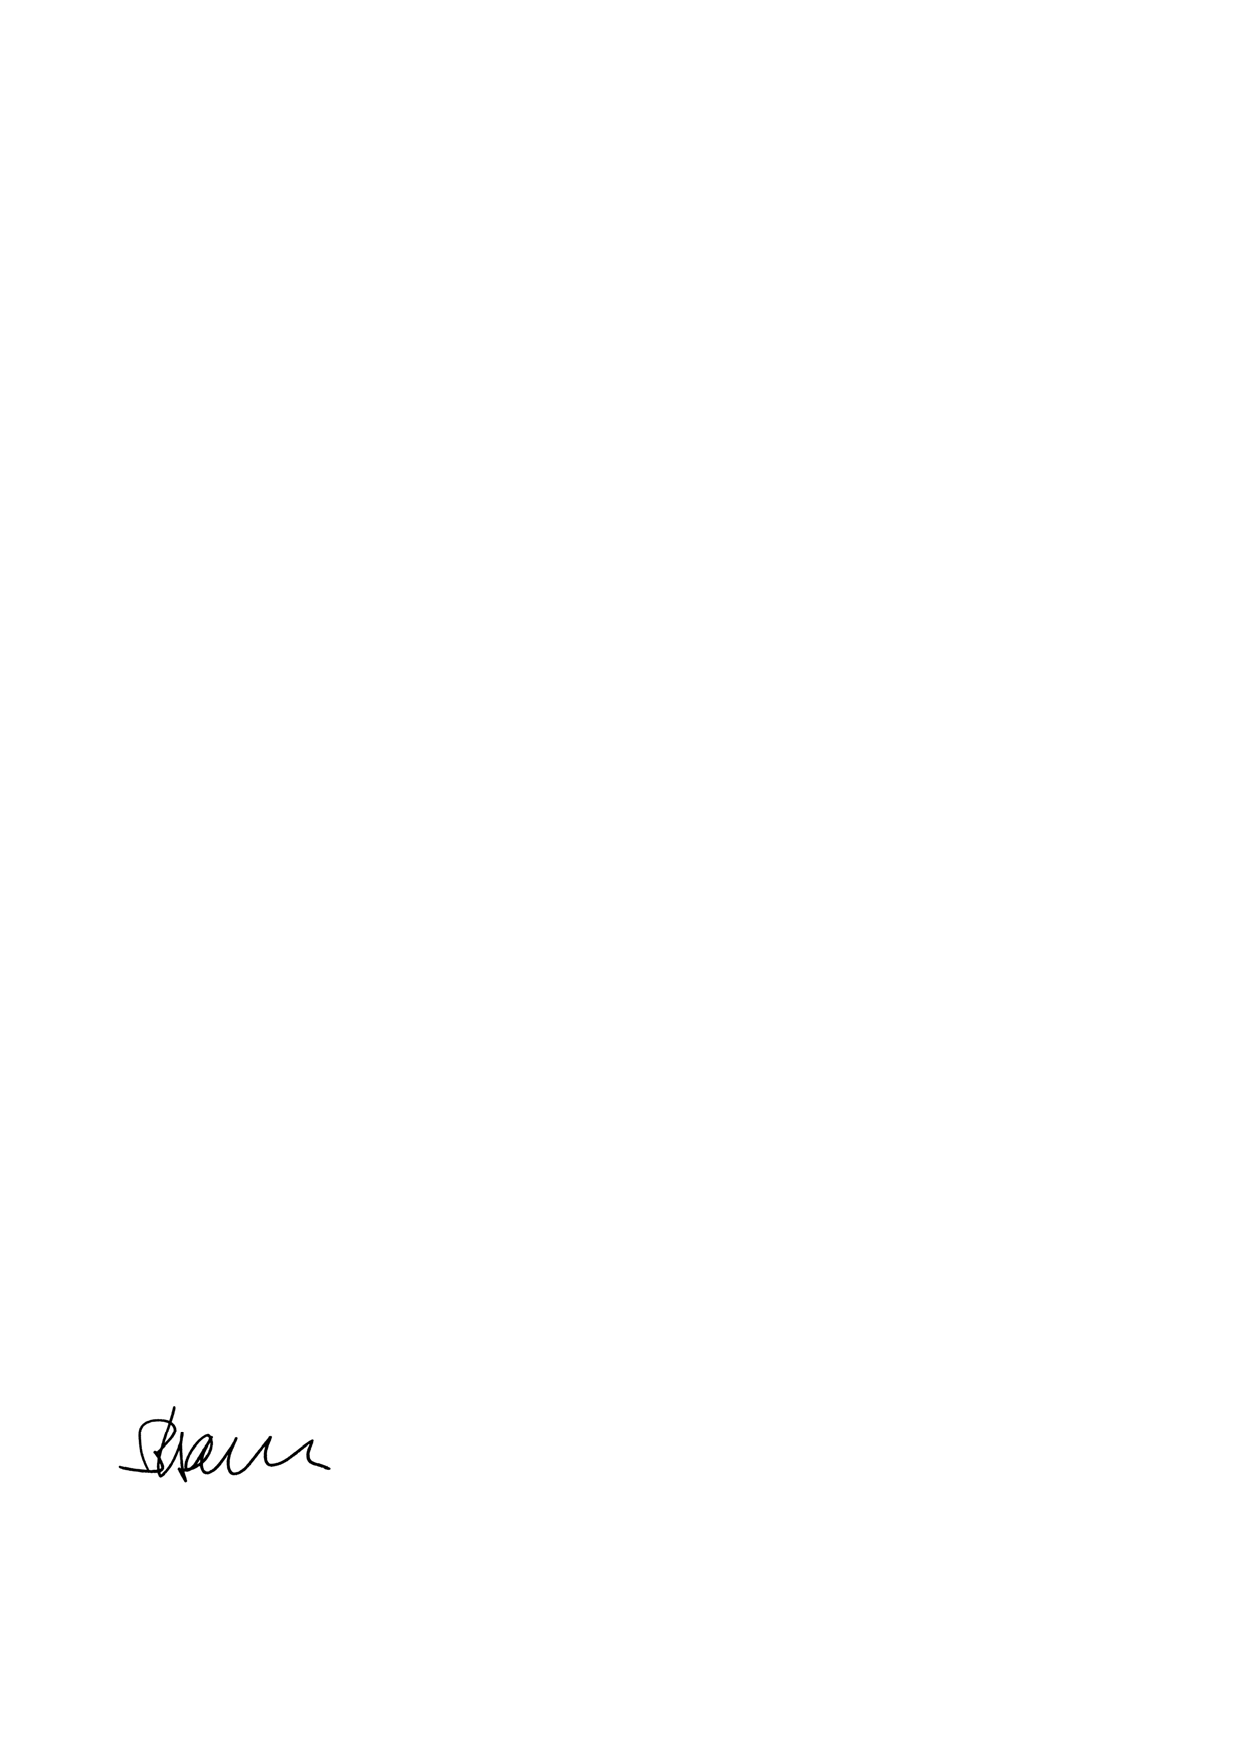
\includegraphics[width=4cm]{DeanSig}
 \end{figure}



Bernhard Kramer

\cleardoublepage
% Each chapter starts on a right page
\shorttitle{Information and Communication Technologies}
\section{Information and Communication Technologies}

The increasing impact of information and communication technology dominates our everyday
life, our society, and the environment.  Examples comprise the World-Wide-Web, the
ubiquitous use of computers, cellular multimedia and wireless communications, robots in
factories as well as in offices and homes, and sophisticated computer models used to
predict the evolution of complex systems such as the global climate.

The enormous level of integration in micro-electronics has enabled unprecedented progress
in many sectors -- and even more importantly, it has created many new profitable
technologies and services based on them. The 21st century will witness technologies that
enable machines to do things that have been so far restricted to humans: machines will be
able to sense, act, speak, listen, decide and sometimes understand. Our T-shirts may have
their own Internet addresses and wirelessly tell the laundry machine about proper
treatment. We will see cars that negotiate with each other in order to maximize traffic
flow while reducing pollution using sophisticated energy management systems. Manufacturing
technologies will improve using a combination of detectors and software to control
processes. Robots are also more and more used in domains where some autonomy and
intelligence is necessary. They work under conditions where it is unpleasant or even risky
for humans like in abandoned mines or at disaster sites and where they have to deal with
situations unforeseen by their designers and programmers. The hallmark of such smart
systems is their integration of technologies from analogue devices and sensors,
communication systems and networks, internet services, artificial intelligence, machine
learning, robotics, and many more.

The School of Engineering and Science actively contributes to this
rapidly growing, boldly interdisciplinary endeavor, focusing on the
areas described in the following.
%
%{\em{Mathematical and Symbolic Modeling}\\
%  \item Reasoning and Semantics
%  \item Simulation and Control of Complex Systems
%  \item Machine Learning
%  \end{itemize}
%\item {\em{Communication Networks and Systems}}, in particular:
%  \begin{itemize}
%  \item Wireless and Cellular Communications
%  \item Digital Transmission Methods and Coding
%  \item Networks and Protocols
%  \item Harmonic Analysis applied to communications engineering
%  \end{itemize}
%\item {\em{Robotics and Embedded Systems}}, in particular:
%  \begin{itemize}
%  \item Robotics
%  \item Applied Algorithms
%  \end{itemize}
%\item {\em{Knowledge and Information Management Systems}}, in
%  particular:
%  \begin{itemize}
%  \item Raster Data Services
%  \item Knowledge Management Systems
%  \item Distributed Systems
%  \item Hierarchical Data Representation
%  \end{itemize}
%\item {\em{Microelectronic Devices and Technologies}}, in particular:
%  \begin{itemize}
%  \item Electronic Devices and Nano Photonics
%  \item Microelectronics
%  \end{itemize}
%\item {\em{Digital Signal Processing}}, in particular:
%  \begin{itemize}
%  \item Signal Processing in Communications
%  \item Nonlinear Signal Processing and Control
%  \end{itemize}
%\end{enumerate}

%%% Local Variables:
%%% mode: latex
%%% TeX-master: "report"
%%% End:

\shorttitle{Communication Networks and Systems}
\subsection{Communication Networks and Systems}

The basic desire of modern society to be able to access and
distribute ``any'' information at ``anytime'' and ``anywhere'' is
the driving force for the rapid development of communication
networks and systems. The implications of these goals are manifold
and require truly interdisciplinary research efforts. A typical, but
clearly not complete, list of involved high level research fields
includes

\begin{myitemize}
\item Wireless Network Engineering and System Design
\item Network Interoperability
\item System capacity management and optimization
\item Information transmission
\item Network protocols 
\item Information security.
\end{myitemize}

All these research areas are strongly inter-related and the strength
of a research cluster in ``communication networks and systems''
resides in the close cooperation of the respected research groups
involved. The particular `flat hierarchy' at IUB (no departments and
chairs) fosters such cooperations.

%%% Local Variables:
%%% mode: stex
%%% TeX-master: "report"
%%% End:




\subsubsection{Cellular and Wireless Communications}
\label{Haas1} \index{Haas, Harald}

\paragraph{Research Team}
Harald Haas (Professor), Rami Abu-Alhiga (PhD Student), Zubin
Bharucha (PhD Student), Hany Elgala (PhD Student), Ellina Foutekova
(PhD Student), Birendra Ghimire (PhD Student), Dennis Kolyuzhnov
(PhD Student),  Raed Youself Mesleh (PhD Student), Abdurazak Mudesir
(PhD Student), Hrishikesh Venkataraman (PhD Student), Sinan
Sinanovic (Research Associate), Peter Omiyi (Postdoc), Mostafa
Afgani (Research Engineer), Sudharasan Ganesan (Graduate Student)\\

Research in Cellular and Wireless Communications is geared towards
new technologies. Particular focus is  on the development and the
interaction of key air-interface building blocks \newpage

\begin{myitemize}
\item multicarrier transmission (in particular OFDM (Orthogonal Frequency Division
Multiplexing)
\item duplexing techniques (in particular time division duplexing
(TDD))
\item multiple-input multiple-output (MIMO) techniques
\item wireless ad hoc systems
\item medium access control (MAC) algorithms
\item multiple access and scheduling techniques
\item dynamic channel assignment (DCA) algorithms
\item mobile positioning
\item visible light communication.
\end{myitemize}

\myparagraph{Highlights} \emph{Spatial Modulation.} Spatial
modulation (SM) is a new and patented multiple antenna transmission
approach for wireless systems that increases the spectral efficiency
(number of bits transmitted per Hz bandwidth) by utilizing the
transmit antenna number as an implicit source of information. A
block of information bits is mapped to an information symbol and a
transmit antenna number. As a consequence, at any given time instant
only a single antenna of the antenna array is transmitting signal
power. The actual block of information bits determines which antenna
is active at a particular time instant. As a result, inter-channel
interference (ICI) at the receiver input and the need to synchronize
the transmit antennas are completely avoided. Simple receiver
algorithms such as maximum receive ratio combining (MRRC) can be
used to retrieve the information bits. The performance and the
receiver complexity of SM and V-BLAST (Vertical-Bell Labs Layered
Space-Time) algorithm in flat fading channels are compared. V-BLAST
applies zero forcing detection based optimum ordering, nulling and
successive interference cancellation. The basic principle of SM is
depicted in Fig.~\ref{smexmpl}, and results of the comparison with
state-of-the-art V-BLAST are shown in Fig.~\ref{fig55}.
\begin{figure}[!htb]\centering
  \centerline{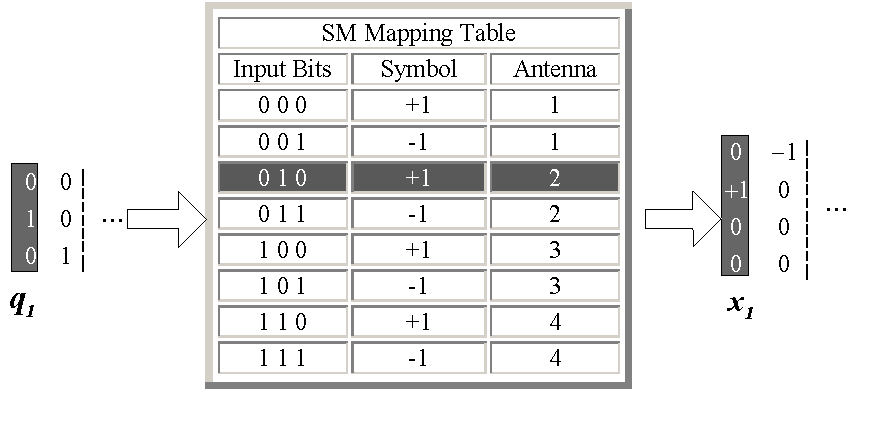
\includegraphics[width=8cm]{haas_1.pdf}}
  \caption{3bits/symbol spatial modulation mapping table using binary phase shift keying (BPSK)
    and four transmit antennas} \label{smexmpl}
\end{figure}
\begin{figure}[!!htp]\centering
  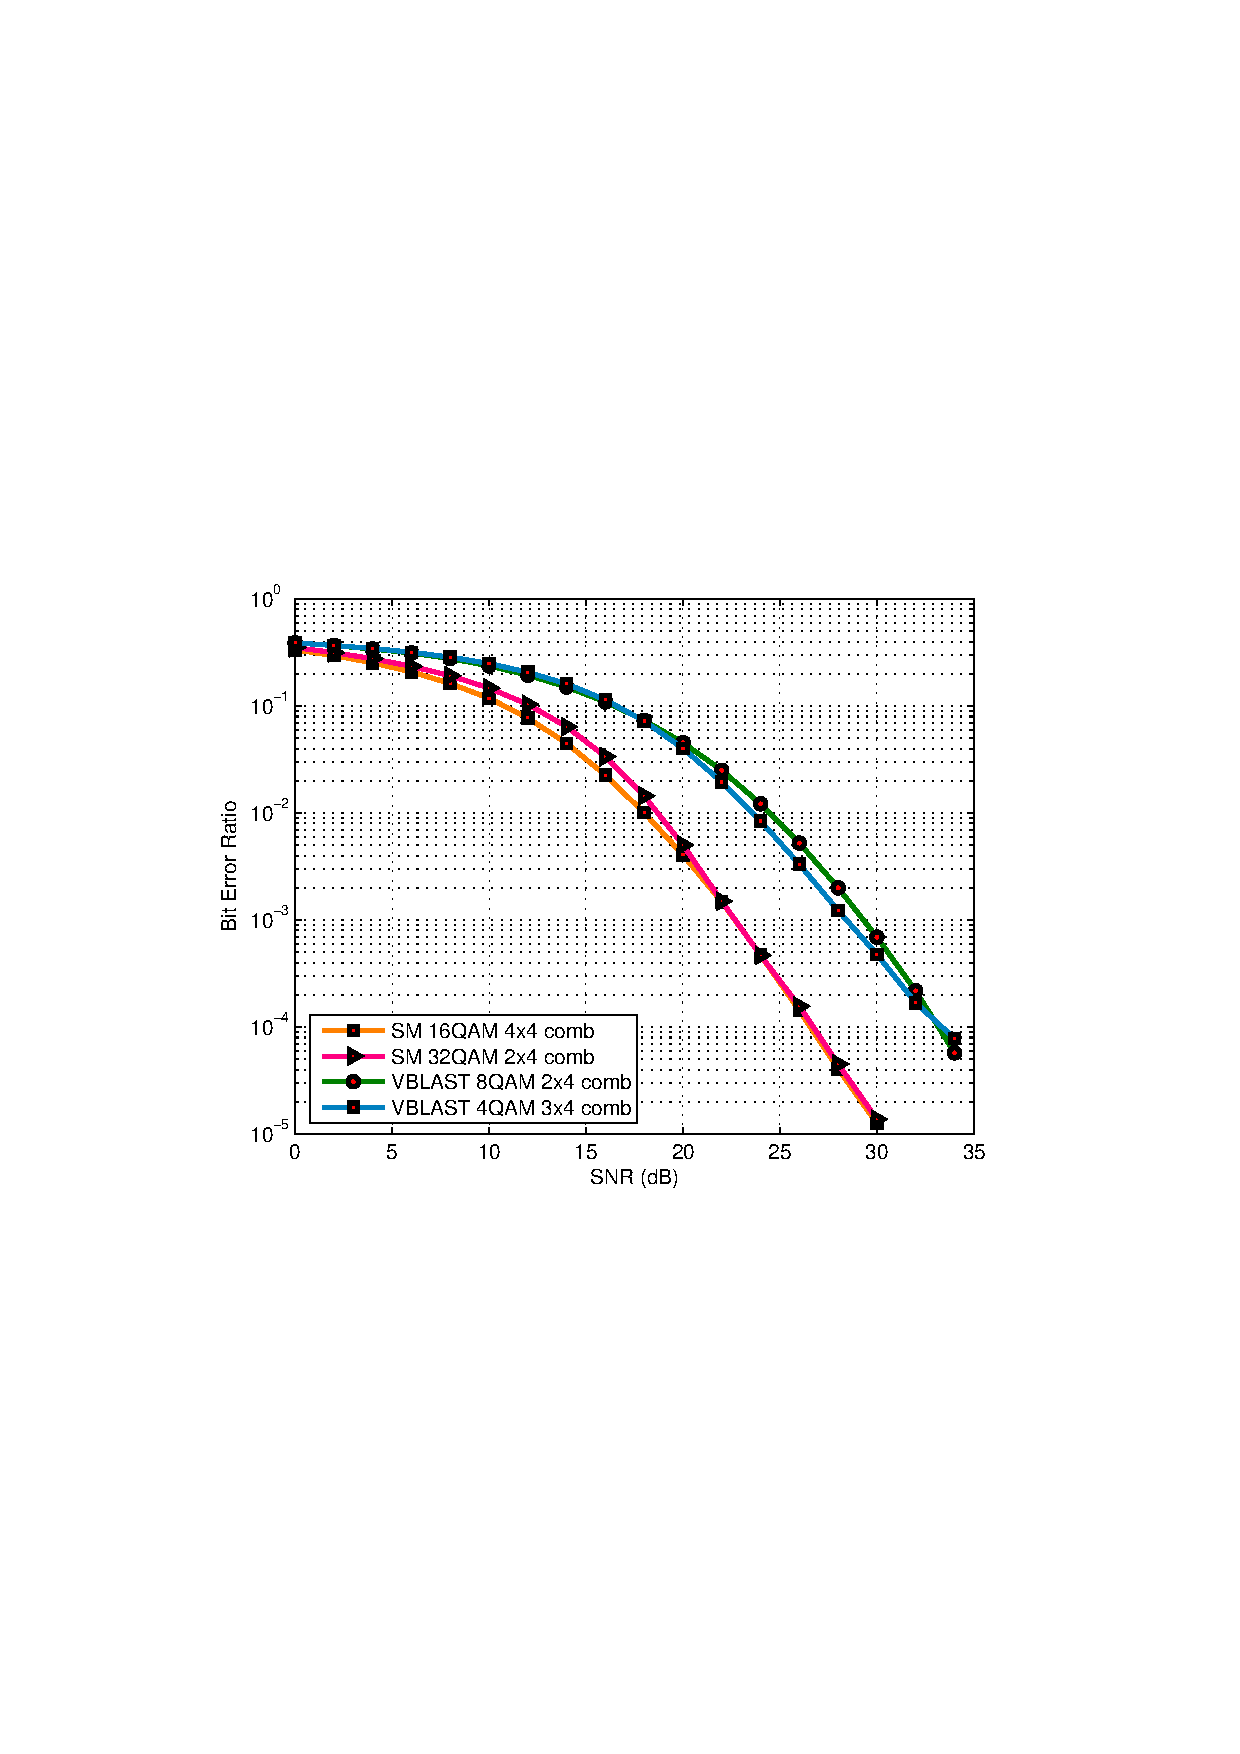
\includegraphics[width=8cm]{haas_2.pdf}\\
  \caption{Bit error performance as a function of signal-to-noise ratio (SNR) for state-of-the-art V-BLAST and novel SM.}
  \label{fig55}
\end{figure}
From the results it can be found that the performance gains are
significant. In both schemes the same number of bit per unit
bandwidth are transmitted (for fair comparison), but with SM the bit
error performance is reduced considerably. For example, at an SNR of
20dB a 10-fold reduction in the BER is observed.

\emph{Dynamic Resource Allocation.} In this work a fully
decentralized interference avoidance algorithm to manage
interference in an \emph{ad hoc} wireless network, applicable to
wireless sensor networks, is developed and analyzed. Fig.~\ref{dca}
depicts a randomly chosen distribution of transmitting (Tx) and
receiving (Rx) nodes. The new algorithm, called \emph{busy tone
interference tolerance signaling}, is of low complexity and is very
easy to implement. It is based on different functions to set the
busy tone signal power dependent on the level of tolerable
interference, and their performance is compared with a special case
of a fixed power system which provides maximum capacity assuming
equal transmit powers. Results show that an appropriately chosen
function for setting the busy-tone can lead to gains in capacity
using very little power. This power efficiency advantage is quite
significant, implying that battery life of units can be extended
while providing a similar capacity than a fixed power system.
\begin{figure}[!!htp]
 \centering
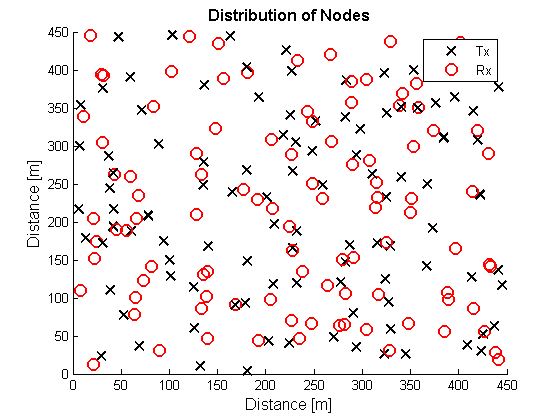
\includegraphics[width=8cm]{haas_3.png}\\
\caption{Random distribution of nodes in an \emph{ad hoc} wireless network}
\label{dca}
\end{figure}

%\null Harald Haas is also involved in ``Signal Processing''
%(Section~\ref{Haas1}).

%\newpage
\paragraph{Organization}
% list the (research) events you have organized, if any,
\begin{enumerate}
    \item Member of Technical Program Committee of and session chair
          at \emph{IEEE International Conference on Personal, Indoor \& Mobile Radio Communications} -- PIMRC 2006
    \item Member of Technical Program Committee of \emph{International IEEE Conference on Vehicular Technology} -- VTC 2006
\end{enumerate}

\paragraph{Collaborations}
\begin{enumerate}
\item {\sl The University of Edinburgh, UK}\\
  Prof. S. McLaughlin\\
  Joint project with industrial partner on \emph{Hybrid Cellular and Multihop Wireless
    Networks}
\end{enumerate}

\newpage
\paragraph{Grants}
% list the running grants in 2005, if none have been received, please delete this
% subsection.
\begin{enumerate}
    \item Funded by industry partner,
      \emph{Cellular TDD-OFDM (Time division duplex - orthogonal frequency
          division multiplexing)},  June 2004 - July 2005


    \item Funding by industry partner and University of Edinburgh, \emph{Hybrid Cellular and Multihop Wireless
    Networks},  July 2005 - July 2006

    \item Funded by industry partner, \emph{Link Adaptation and Scheduling in Cellular
    Systems},  March 2005 - February 2008

    \item Funded by Bremen T.I.M.E program funded by BIS
    Bremerhaven, \emph{Mobile Positioning (MPos)} in collaboration with MobilTec GmbH and supported by
     T-Mobile,  June 2006 - September 2009

    \item Funded by DFG Schwerpunktprogram TakeOFDM, \emph{DCA Algorithms and MAC Protocols for COFDM Based Cellular and
     Ad hoc Systems Using Carrier Sensing Time Division Multiple Access
     (CSTDMA)},  October 2004 - September 2006

\end{enumerate}

\paragraph{Patents}
% list the grants you have received in 2005, if none have been received, please delete this
% subsection.
\begin{enumerate}
\item Four new patent applications submitted
\item Three previously submitted patents got granted in 2006
\end{enumerate}

\paragraph{Awards, Prizes}
\begin{enumerate}
\item Nominated for the Chinese 111 Program -- Guest Academic Talents Programme for the Development of University Disciplines in China
\item Invited Talk at the University of Mondragon (Spain)
%    \item Honorary Fellowship of Edinburgh University
%    \item Invited to Institute for Digital Communications (IDCOM) at the University of
%          Edinburgh on \emph{Vodafone Fellowship on Communications}
    %\item Invited speaker at \emph{International Next Generation Wireless Network Workshop},
     %     Edinburgh/Scotland
\end{enumerate}

%\paragraph{Publications}
% list the publications of 2005 (also accepted and in press), if none have been received, please delete this
% subsection. Enter the publications into the SES publications database at
% http://kwarc.eecs.iu-bremen.de/ses-pubs/index.php and only reference them here.

 
\nocite{ah06_vis_light}
\nocite{bh06_ped_dead_reck}
\nocite{hnona06_iamac}
\nocite{vh06_thru_cap}
\nocite{cvh06_freq_syn}
\nocite{feh06_semi_analytic}
\nocite{fagvh06_sch_CDMA}
\nocite{jhm06_adhoc_tdd_underlay}
\nocite{oha06_tsalloc_insotdd}
\nocite{mhay06_spatialmod}
\nocite{asilomar06}
\nocite{chinacom06}
\nocite{tdd_book}
\nocite{oha07}
 

 
\begin{bibunit}[hplain]
\begin{thebibliography}{10}

\bibitem{ah06_vis_light}
M.~Afgani and H.~Haas.
\newblock Visible light communication using {OFDM}.
\newblock In {\em Proceedings of the 2nd International Conference on Testbeds
  and Research Infrastructures for the Development of Networks and Communities
  (Trident 2006)}, Barcelona, Spain, March 01-06 2006.

\bibitem{bh06_ped_dead_reck}
S.~Beauregard and H.~Haas.
\newblock "{Pedestrian Dead Reckoning (PDR) and GPS for Indoor Positioning}".
\newblock In {\em Proceedings of 3rd Workshop on Positioning, Navigation and
  Communication ({WPNC}'06)}, Hannover, Germany, March 16 2006.

\bibitem{cvh06_freq_syn}
S.~Chaudhury, H.~Venkataraman, and H.~Haas.
\newblock "{Uplink Capacity Comparison of Non-Perfect Frequency Synchronised
  Cellular OFDM Systems}".
\newblock In {\em Proceedings of International Wireless Communications and
  Mobile Computing Conference ({IWCMC} 2006)}, Vancouver (Canada), July 3-6
  2006.

\bibitem{fagvh06_sch_CDMA}
E.~Foutekova, P.~Agyapong, B.~Ghimire, H.~Venkataraman, and H.~Haas.
\newblock "{Scheduling in Cellular TDD-CDMA Networks}".
\newblock In {\em Proceedings of the International Vehicular Technology
  Conference ({VTC}) 2006-Fall}, Montreal, Canada, September 25-28 2006. IEEE.

\bibitem{feh06_semi_analytic}
E.~Foutekova, C.~Evers, and H.~Haas.
\newblock "{Semi-Analytical Derivation of Interference in TDD-CDMA Systems
  Employing Random Time Slot Hopping (RTSH)}".
\newblock In {\em Proceedings of the International Vehicular Technology
  Conference ({VTC}) 2006-Fall}, Montreal, Canada, September 25-28 2006. IEEE.

\bibitem{asilomar06}
S.~Ganesan and H.~Haas.
\newblock "{On the Performance of Spatial Modulation OFDM}".
\newblock In {\em "{Asilomar Conference on Signals, Systems, and Computers}"},
  Monterey, CA, USA, October 30 -- November 1 2006. IEEE.

\bibitem{hnona06_iamac}
H.~Haas, V.~D. Nguyen, P.~Omiyi, N.~H. Nedev, and G.~Auer.
\newblock "{Interference Aware Medium Access in Cellular OFDMA/TDD Network}".
\newblock In {\em Proceedings of International Conference on Communications
  ({ICC} 2006)}, Istanbul, Turkey, June 11-15 2006. IEEE.

\bibitem{tdd_book}
H.~Harald and S.~McLaughlin, editors.
\newblock {\em "{Next Generation Mobile Access Technologies: Implementing
  TDD}"}.
\newblock Cambridge University Press, Spring 2007.

\bibitem{jhm06_adhoc_tdd_underlay}
P.~Jain, H.~Haas, and S.~McLaughlin.
\newblock "{Capacity Enhancement using Ad Hoc Pico-Cells and TDD Underlay}".
\newblock In {\em Proceedings of the 17th International Symposium on Personal,
  Indoor and Mobile Radio Communications ({PIMRC} 2006)}, page~5, Helsinki,
  Finland, September 11-14 2006. IEEE.

\bibitem{mhay06_spatialmod}
R.~Mesleh, H.~Haas, C.~C. Ahn, and S.~Yun.
\newblock "{Spatial Modulation -- OFDM}".
\newblock In {\em Proceedings of the International {OFDM} Workshop}, Hamburg,
  Germany, August 30-31 2006.

\bibitem{chinacom06}
R.~Mesleh, H.~Haas, C.~Wook Ahn, and S.~Yun.
\newblock "{Spatial Modulation -- A New Low Complexity Spectral Efficiency
  Enhancing Technique}".
\newblock In {\em "{ChinaCOM 2006}"}, Beijing, China, October 25 -- 27 2006.
  IEEE.

\bibitem{oha06_tsalloc_insotdd}
P.~Omiyi, H.~Haas, and G.~Auer.
\newblock "{Analysis of Intercellular Timeslot Allocation in Self-Organising
  TDD Cellular Mobile Systems}".
\newblock In {\em Proceedings of the 17th International Symposium on Personal,
  Indoor and Mobile Radio Communications ({PIMRC} 2006)}, page 5 pages on CD
  ROM, Helsinki, Finland, September 11-14 2006. IEEE.

\bibitem{vh06_thru_cap}
H.~Venkataraman and H.~Haas.
\newblock "{Throughput Capacity for 2-Hop Hybrid Cellular Networks}".
\newblock In {\em Proceedings of 6th Scandinavian Workshop on Wireless Ad-hoc
  Networks ({ADHOC} '06)}, Stockholm (Sweden), May 3-4 2006.

\end{thebibliography}
\end{bibunit}
\subsubsection{Digital Transmission Methods and Coding}
\label{ict:cns:henkel} \index{Henkel, Werner}

\paragraph{Research Team}
Werner Henkel (Professor), Fangning Hu (PhD Student), Neele von Deetzen (PhD
Student), Khaled Shawky Hassan (PhD Student), Apirath Limmanee (PhD Student)\\

We currently concentrate on iterative decoding and unequal error protection in
coding and physical transport. In iterative decoding, we study the convergence
behavior and properties of analog Turbo-like codes and the possible design of
Turbo and LDPC codes for unequal error protection (UEP). In the design of UEP
codes, we especially cooperate with ENSEA, France, and Lule\aa\ University,
Sweden. UEP is also the goal in our multicarrier research, where we design
bit-allocation algorithms that allow for easy realization of different
protection classes in an arbitrary way. UEP will be a must for current and
especially future triple-play data services to different devices at varying
channel qualities.

The analog codes have a strong relation to signal processing. Regarding
practical applications of such codes, we especially look into the correction
of impulse-noise and clipping effects. There, the most important task is to
determine statistical properties that allow for easy erasure marking, which
would support further decoding steps, analog and digital.

We further started a project on data transmission using ultrasound signals. We
currently design lab experiments to deliver data for later modeling of the
channel and disturbances.

%%% give a very short (150 words description of your research area)
%% Hint: this can be copied from the research areas document (../masterplan/research-areas)

\paragraph{Highlights}

The design of UEP Turbo codes by a pruning approach led us to a structure that
we named hybrid concatenation, a combination of outer parallel and inner
serial concatenation. The study of the decoding convergence with so-called EXIT
charts yielded the result that the area between the curves describing the
outer iterations depend on the number of inner iterations. This allows for
minimizing the decoding complexity by a scheduling with varying number of
iterations in the different decoding steps (see Fig.~\ref{fig:henkel_1}). The
pruning concept was also the starting point for our design of UEP LDPC codes
with an irregular check-node profile (pat. pending).

\begin{figure}[ht]
  \centering
  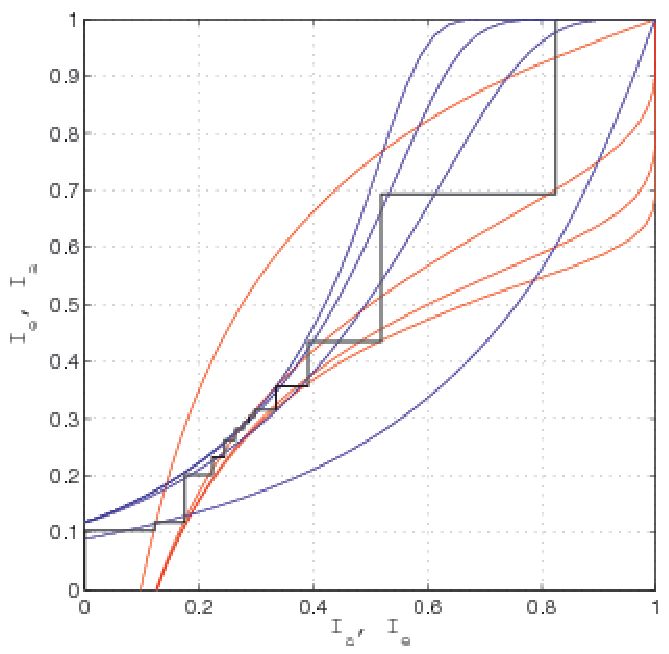
\includegraphics[width=7cm]{henkel_1}
 \caption{Convergence scheduling for hybrid concatenation}
%  \caption{Convergence scheduling for hybrid concatenation}
  \label{fig:henkel_1}
\end{figure}

In analog coding, we further improved the presentation of our proof that
Turbo-like decoding leads to a least-squares solution. We can now exactly
forecast the convergence limits for the stepsize and can also
modify it for every iteration to allow for very fast
convergence. For impulse-noise detection, we currently investigate new
statistical properties, e.g., the slope distribution, and correlation
approaches. This study will also close a gap in impulse-noise modeling
regarding the autocorrelation function of impulse noise.

By designing a new bit-allocation algorithm (pat. pending), following the
principles of an existing one by Chow, Cioffi, and Bingham, we can obtain UEP
properties in a very elegant way. It allows for an arbitrary number of
error-protection classes with arbitrary margins between them and an arbitrary
number of bits per class. Figure~\ref{fig:henkel_2} shows a resulting bit and
power allocation according to the channel SNRs, assuming three error protection
classes with a 3 dB separation.


\begin{figure}[ht]
  \centering
  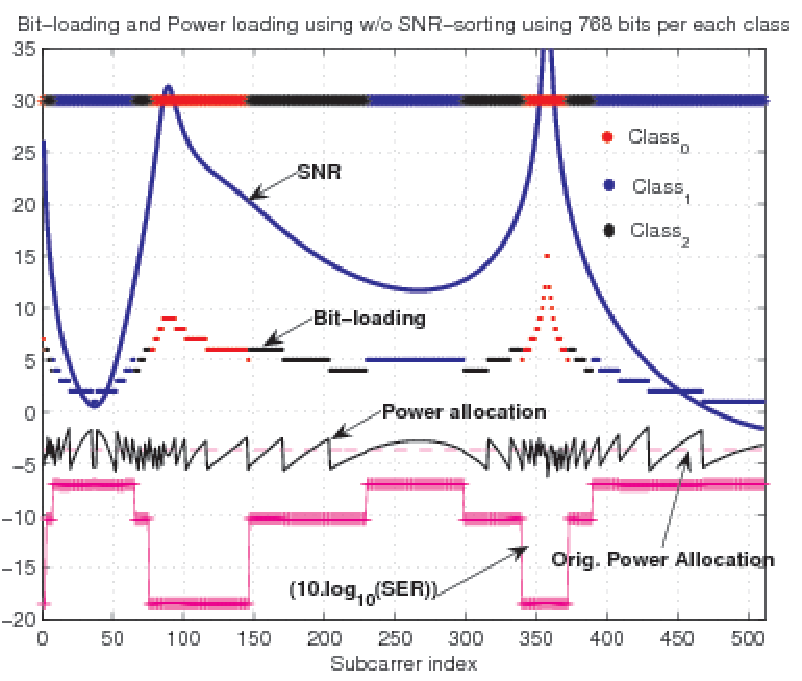
\includegraphics[width=7cm]{henkel_2}
  \caption{UEP bit and power allocation for three protection classes}
%  \caption{UEP bit and power allocation for three protection classes}
  \label{fig:henkel_2}
\end{figure}

\newpage
\paragraph{Organization}
% list the (research) events you have organized, if any,

\begin{enumerate}
\item Program Committee member of ICC 2006
\end{enumerate}

%\paragraph{Collaborations}
%\begin{enumerate}
%\item ...
%\item ...
%\item ...
%\end{enumerate}

\paragraph{Grants}
% list the running grants in 2005, if none have been received, please delete this
% subsection.
\begin{enumerate}
\item Funded by EU-IST STREP (FP 6), \emph{M-Pipe}, (October 2004
- March 2007)
\end{enumerate}

\paragraph{Patents}
\begin{enumerate}
\item  L. Sassatelli, W. Henkel, and D. Declercq. Check-Irregular LDPC Codes, Jan. 27
  2006. European Patent Application 06 100 979.1.
\item W. Henkel and K. Hassan. Unequal Error Protection Bit Loading for Multi-Carrier
  Transmission, Aug 30 2006. European Patent Application 06 119 771.1.
\end{enumerate}


%\paragraph{Publications}
% list the publications of 2005 (also accepted and in press), if none have been received, plese delete this
% subsection. Enter the publications into the SES publications database at
% http://kwarc.eecs.iu-bremen.de/ses-pubs/index.php and only reference them here.

%\begin{description}

%\item[Conference Proceedings]
  \nocite{Henkel_vDeetzen_IZS}
  \nocite{Hu_Henkel_Turbo}
  \nocite{Sassatelli_Henkel_Declercq_Turbo}
  \nocite{vDeetzen_Henkel_ISIT}
  \nocite{Henkel_Hassan_OFDM}
  \nocite{vDeetzen_ITG}
  \nocite{Hassan_Henkel_ITG}
%\item[Patents]
%  \nocite{Sassatelli_Henkel_Declercq_EP}
%  \nocite{Henkel_Hassan_EP}
%\end{description}

%%% Local Variables:
%%% mode: latex
%%% TeX-master: "report"
%%% End:

 \begin{bibunit}[hplain]\begin{thebibliography}{1}

\bibitem{Hassan_Henkel_ITG}
K.~Hassan and W.~Henkel.
\newblock {Unequal Error Protection Bit Loading in MIMO OFDM}.
\newblock In {\em ITG-Fachgruppe, 8. Sitzung}, Bremen, Oct. 6 2006.

\bibitem{Henkel_Hassan_OFDM}
W.~Henkel and K.~Hassan.
\newblock {OFDM (DMT) Bit and Power Loading for Unequal Error Protection}.
\newblock In {\em OFDM Workshop}, Hamburg, Aug 30-31 2006.

\bibitem{Henkel_vDeetzen_IZS}
W.~Henkel and N.~von Deetzen.
\newblock {Path Pruning for Unequal Error Protection Turbo Codes}.
\newblock In {\em 2006 International Z\"urich Seminar on Communications},
  Z\"urich, Switzerland, Feb. 22-24 2006.

\bibitem{Hu_Henkel_Turbo}
F.~Hu and W.~Henkel.
\newblock {A Geometric Description of the Iterative Least-Squares Decoding of
  Analog Block Codes}.
\newblock In {\em 4th International Symposium on Turbo Codes \& Related Topics
  in connection with the 6th International ITG-Conference on Source and Channel
  Coding}, Munich, April 4-7 2006.

\bibitem{Sassatelli_Henkel_Declercq_Turbo}
L.~Sassatelli, W.~Henkel, and D.~Declercq.
\newblock {Check-Irregular LDPC Codes for Unequal Error Protection under
  Iterative Decoding}.
\newblock In {\em 4th International Symposium on Turbo Codes \& Related Topics
  in connection with the 6th International ITG-Conference on Source and Channel
  Coding}, Munich, April 4-7 2006.

\bibitem{vDeetzen_ITG}
N.~von Deetzen.
\newblock {Decoder Scheduling of Hybrid (parallel/serial) Turbo Codes}.
\newblock In {\em ITG-Fachgruppe, 7. Sitzung}, Munich, May 22 2006.

\bibitem{vDeetzen_Henkel_ISIT}
N.~von Deetzen and W.~Henkel.
\newblock {Decoder Scheduling of Hybrid Turbo Codes}.
\newblock In {\em 2006 IEEE International Symposium on Information Theory (ISIT
  2006)}, Seattle, Washington, USA, July 9-14 2006.

\end{thebibliography}
\end{bibunit}

\onecolumn

\section{Education}
The School of Engineering and Science offers 12 Bachelor of Science
programs

\begin{myitemize}
\item Mathematics
\item Physics
\item Chemistry
\item Biology

\item Biochemical Engineering
\item Biochemistry and Cell Biology
\item Bioinformatics and Computational Biology
\item Geosciences and Astrophysics
\item Computer Science
\item Electrical and Computer engineering
\item Electrical Engineering and Computer Science
\end{myitemize}
\ \ \\
 and seven Master's programs
\ \ \\
\begin{myitemize}
\item Mathematical Sciences
\item Astroparticle Physics
\item Biological Recognition
\item Nanomolecular Science
\item Geo-Ocean Dynamics
\item Communications, Systems and Electronics (Electrical
Engineering)
\item Smart Systems (Computer Science.)
\end{myitemize}


\subsection{Master's Degrees}\shorttitle{MSc Degrees}
\paragraph{Biological Recognition}
\begin{enumerate}
    \item {\sl  Esther  Ghanem:}    `` Hetrologous expression of murine tapasin in the yeast expression systems S.cerevisiae and P.pastoris" \\ Examiners:     Prof. Dr. Albert Jeltsch,   Prof. Dr. Sebastian Springer
    \item {\sl  Srinivasaraghavan   Kannan:} ``Enhanced Conformational sampling of peptides and proteins by Biasing potential Replica Exchange Molecular Dynamics Simulations (BP - REMD)" \\ Examiners:     Prof. Dr. Martin Zacharias,   Prof. Dr. Mathias Winterhalter
    \item {\sl  Rustem  Khusainov :}      ``On the facilitation of dye-affinity sorption methods for Downstream Processing of bioproducts" \\ Examiners:     Prof. Dr. Marcelo Fernandez-Lahore  ,   Prof. Dr.Mathias Winterhalter
    \item {\sl  Liliya  Kulishova :}      ``Investigation of the Residues Involved in Target Sequence Recognition by the M.EcoRV Adenine-N6-methyltransferase" \\ Examiners:     Prof. Dr. Albert Jeltsch    ,   Prof. Dr. Ulrich Schwaneberg
    \item {\sl  Benny   Mwale:}    ``Encapsulation and Characterization of Horseradish Peroxidase in Liposomes" \\ Examiners:     Prof. Dr. Mathias Winterhalter,   Prof. Dr. J�rgen Fritz
    \item {\sl  Rakina  Yaneva:}   `` Cloning, expression, and purification of murine tapasin in E. coli" \\ Examiners:     Prof. Dr. Martin Zacharias,   Prof. Dr. Sebastian Springer

\end{enumerate}
\paragraph{Communications, Systems and Electronics}
\begin{enumerate}
    \item {\sl  Mostafa Afgani: } ``On User Scheduling in the Downlink of a Cellular OFDMA System" \\ Examiners:     Prof. Dr. Harald Haas,   Dr. Gunther Auer
    \item {\sl  Sudharsan   Ganesan: } ``On the Performance of Spatial Modulation OFDM" \\ Examiners:     Prof. Dr. Harald Haas,   Dr. Mathias Bode
     \item {\sl  Abdurazak   Mudesir: } ``Analytical derivation of the pdf of the signal to interference ratio(SIR) in a cross layer environment under Nakagam-m distribution fading envelop. " \\ Examiners:     Prof. Dr. Harald Haas,    Dr. Mathias Bode
    \item {\sl  Nandhavel   Sethubalasubramanian: } ``Design of low power SIMD shufflers using Datapath Generator " \\ Examiners:     Prof. Dr. Werner Bergholz,   Dr. Franky Catthoor
\end{enumerate}
\paragraph{Geo-Ocean Dynamics}
\begin{enumerate}
    \item {\sl  Serkan  Kulkaksiz: } ``The Bahviour of Anthropogenic Gd in Comparison with Natural Rare Earth Elements and Yttrium in the Weser Estuary" \\ Examiners:     Prof. Dr. Michael Bau,   Prof. Dr. Andrea Koschinsky-Fritsche
    \item {\sl  Prasesh Sharma: } ``Potential correlation of heavy metal contamination in surface soils with infestation of viscum album in poplar trees in Goslar using a micro-ecosystem study" \\ Examiners:     Prof. Dr. Andrea Koschinsky-Fritsche,   Prof. Dr. Dr. Ewald Schnug
    \item {\sl  Aryani  Sumoondur: } ``Amino acids and primary amines in seawater and hydrothermal fluids from the Mid-Atlantic Ridge: Implications for metal-amino acid interactions" \\ Examiners:     Prof. Dr. Andrea Koschinsky-Fritsche,   Dr: Christian Ostertag-Henning
\end{enumerate}

\paragraph{Nanomolecular Science}
\begin{enumerate}
    \item {\sl  Supriya Babu: } ``Novel methods of preparation of Liposome-Based Nanocapsules" \\ Examiners:     Prof. Dr. Mathias Winterhalter,   Prof. Dr. J�rgen Fritz
    \item {\sl  Tivadar Mach: } ``Translocation through nanopores via an internal binding site" \\ Examiners:     Prof. Dr. Mathias Winterhalter,   Prof. Dr. J�rgen Fritz
    \item {\sl  Ahson   Shaikh: } ``One-Pot Asymmetric Sequential Amination-Alkylation Methodology: Synthesis of Chiral Amines" \\ Examiners:     Prof. Dr. Thomas Nugent,   Prof. Dr. Werner Nau
\end{enumerate}

\paragraph{Smart Systems}
\begin{enumerate}
   \item {\sl  Horia   Balan: } ``An Experimental Evaluation of
Voice-over-IP Quality over the Datagram Congestion Control Protocol"
\\ Examiners:     Prof. Dr. J�rgen Sch�nw�lder, Prof. Dr. Michael
Kohlhase  ,   Dr. Lars Eggert
\item {\sl  Hamed   Bastani: } ``Absolute 3D Indoor Radio Positioning
Using Dynamic Roles Assignment" \\ Examiners:     Prof. Dr. Stefano
Carpin,   Prof. Dr. Harald Haas
\item {\sl
Gorkem  Erinc: } ``Nonholonomic Motion Planning Using Genetic
Algorithms for Car-Like Robots" \\ Examiners:     Prof. Dr. Stefano
Carpin,   Prof. Dr. Andreas Birk

 \item {\sl Andreas Kolling: } ``Multirobot Cooperation for Surveillance of
Multiple Moving Targets - An Improved Behavioral Approach and Its
Formalization" \\ Examiners:     Prof. Dr. Stefano Carpin, Prof. Dr.
Herbert Jaeger
   \item {\sl  Seongchu    Lee: } ``Localization
and map building in volumetric modeling for autonomous mobile robots
" \\ Examiners:     Prof. Dr. Andreas Birk, Prof. Dr. Stefano Carpin
   \item {\sl  Mantas Lukosevicius: } ``
Improving Echo State Networks by Training Intermediate Units" \\
Examiners:     Prof. Dr. Herbert Jaeger ,   Dr. Mathias Bode
\end{enumerate}


\shorttitle{PhD Degrees} \subsection{PhD Degrees}

\paragraph{Mathematical Sciences}

\begin{enumerate}
\item {\sl Alexandra Kaffl:}
 ``Hubbard Trees and Kneading Sequences for Unicritical and Cubic Polynomials''
\\ Dissertation Committee: Prof. D.
Schleicher (supervisor), Prof. M. Stoll, Prof. R. O. Wells, Prof. J.
Milnor, Prof. M. Rees, Prof. H. Bruin
\item {\sl Johannes R\"{u}ckert:}
``Newton's Method as a Dynamical System''
\\ Dissertation Committee: Prof.  D. Schleicher (supervisor), Prof. M. Oliver, Prof.
R. O. Wells, Prof. M. Lyubich, Prof. H. Bruin
\end{enumerate}

\paragraph{Chemical Sciences}

\begin{enumerate}
\item {\sl Firasat Hussain:}
``Hybrid Organic-Inorganic Polyoxometalates Functionalized by
Diorganotin Groups''
\\ Dissertation Committee: Prof. U. Kortz (supervisor), Dr. M. Dickmann,
Prof. E. Cadot, Prof. M. Pope
\item {\sl Annette Wensing:}
 ``Siderophore Production of {\sl Pseudomonas syringae} and its Implications
 on the Biological Control of Bacterial Blight of Soybean''  \\
 Dissertation Committee: Prof. M. Ullrich (supervisor), Prof. U.
Schwaneberg, Prof. G. Muskhelishvili, Prof. B. V\"{o}lksch
\item {\sl Alexander Kraynov:}
    ``Preparation and Characterization of Pt and Pd Nanoclusters Modified with
    Chiral Ligands: Examination of Catalytic Activity in Hydrogenation of Ethyl
    Pyruvate'' \\ Dissertation Committee: Prof. R. Richards (supervisor), Prof.
T. Nugent, Prof. S. Tautz
\item {\sl Harekrushna Sahoo:}
   ''Investigation of Structural, Conformational, and Dynamic
   Properties of Polypeptide by Fluorescence-Based Techniques''
   Dissertation Committee: Prof. W. Nau (supervisor), Prof. M.
   Zacharias, Prof. T. Nugent, Prof. X. Zang
\item {\sl Tuck Seng Wong:}
   ''Expanding the Toolbox of Directed Evolution for Understanding
   Protein Structure-Function Relationships''
   Dissertation Committee: Prof. U. Schwaneberg (supervisor), Dr. D.
   Roccatano, Prof. M. Zacharias, Prof. K-E. Jaeger
\end{enumerate}

\paragraph{Life Sciences}

\begin{enumerate}
\item {\sl Kristina Mayer:} ``Cathepsins during Intestinal Trauma''
\\ Dissertation Committee: Prof. K. Brix (supervisor), Prof. A. Lerchl, Prof.
A. Baici
\item {\sl Silvia Jordans:}
 ``Localization, Trafficking and functional Role of Cysteine Cathepsins in Thyroid Epithelial Cells'' \\
Dissertation Committee:   Prof. K. Brix (supervisor), Dr. D. Buttle,
Prof. A. Lerchl
\item  {\sl Brit Wolters:}
    ``Cathepsins L and V in human Keratinocytes''
\\ Dissertation Committee:  Prof. K. Brix (supervisor),
Prof. M. Ullrich, Prof. A. Lerchl, Dr. D. Buttle
\item {\sl Heiko B\"{u}th:}
 ``Contribution of Lysosomal Cystein Protease Cathepsin B to Extracellular Matris
 remodeling during Keratinocyte Migration and Wound Healing''
\\ Dissertation Committee: Prof. K. Brix (supervisor), Prof.
Boukamp, Prof. A. Lerchl, Prof. M. Ullrich
\item {\sl Karen Hinsch:}
 ``Analysis of Proliferation, Fate and Stem Cell Characteristics of Newly Generated
 Cells in the Adult Fish Brain''
\\ Dissertation Committee: Prof. G. K. H Zupanc (supervisor), Prof.
C. Hilgetag, Prof. S. Thanos
\item {\sl Marcus Lindemann:}
 ``Membrane-Protein Matrix for Technical Application''
\\ Dissertation Committee: Prof. M. Winterhalter (supervisor), Prof. J. Fritz,
Prof. V. Wagner, Prof. E. Schleif
\item {\sl Hong Qu:} ``Significance of Cathepsins B, D and L for Homeostasisof the Small Intestine''
\\ Dissertation Committee: Prof. K. Brix (supervisor), Prof. S. Springer, Prof. M. Ullrich,
Prof. G. van Echten-Deckert
%\item {\sl Mouyu Yang:}
%   ``An Investigation of the Relationships among Light, Vision Signal and Reproduction
%   on Specified Vertebrates and Invertebrates'' \\ Dissertation Committee:
%   Prof. A. Lerchla (supervisor), Prof. K. Brix, Prof. M. Bergmann
\item {\sl Christian Keithahn:}
   ''Radical Scavenging Behavior of Biogenic Amines'' \\
   Dissertation Committee: Prof. A. Lerchl (supervisor), Prof. K.
   Brix, Prof. M. Zacharias, Prof. L. Rensing
\item {\sl Chris Andr\'{e} W\"{u}rdemann:}
   ''Method Development for Expression Profiling in Prokaryotes and
   their Application in Marine Environments'' \\
   Dissertation Committee: Prof. F. O. Gl\"{o}ckner (supervisor), Prof. G.
   Muskhelishvili, Prof. M. Ullrich, Prof. R. Amman
\item {\sl Ziwei Zhu:}
   ''Making Glucose Oxidase fit for Biofuel Cell Applications by
   Directed Protein Evolution''
   Dissertation Committee: Prof. U. Schwaneberg (supervisor), Prof.
   M. Zacharias, Prof. M. Fernandez-Lahore, Prof. V. Hass
\item {\sl Joana Pereira da Silva Gomes:}
   ''Liposomes for Biosensing''
   Dissertation Committee: Prof. M. Winterhalter (supervisor), Prof.
   J. Fritz, Prof. D. Gabel
\item {\sl Stoyan Kurtev:}
   ''Lateralization of Spatial Attention in Human Brain: A 'Virtual Lesion' Approach''
   Dissertation Committee: Prof. C. Hilgetag (supervisor), Prof. B. Olk, Prof. Valero-Cabre
\end{enumerate}


 \newpage
\shorttitle{The School of Engineering and Science}
\section{The School of Engineering and Science}
\subsection{Administration}
\shorttitle{Administration of the School of Engineering and Science}
\begin{tabular}{ll}
Prof. Dr. Kramer, Bernhard &Vice President and Dean \\
 Dr. Allner, Anke
 & Director, Dean's Office \\ Schreiber, Angela  & Assistant to
the Dean \\ Buck, Iris  & Graduate Admission \\
 Dr. Frischholz, Svenja
& Graduate Student Affairs \\
 Knoop, Katja & Team Assistant to the
Faculty \\
 Manss, Sigrid  & Team Assistant to the Faculty \\
 Pankratz, Elke
&Team Assistant to the Faculty
\end{tabular}

\subsection{Advisory Board}
\begin{tabular}{ll}
  Prof. Dr. Andrew S. Douglas (Chair)  & Johns Hopkins University, Baltimore, MD \\
 Prof. Dr. med.
Hans-Jochen Heinze & Otto-von-Guericke-Universit�t, Magdeburg\\
Prof. Dr. Gotthilf Hempel & Bremen \\
 Prof. Dr. James L. Kinsey & William Marsh Rice University, Houston, TX\\
  Prof. Dr. Berrien Moore
III,  & University of New Hampshire \\ Prof. Dr. Heinz-Otto Peitgen
& MeVis, Bremen \\ Prof. Dr. Klaus Pinkau &M�nchen \\ Prof. Dr.
Manfred T. Reetz & Max-Planck-Institut f�r Kohlenforschung,
M�hlheim/Ruhr \\ Prof. Dr. Karl Wieghardt & Max-Planck-Institut f�r
Strahlenchemie, M�hlheim/Ruhr \\
\end{tabular}

\shorttitle{Faculty} \subsection{Faculty}
\begin{longtable}{ll}
Antoulas, Athanasios C., Ph.D.&Visiting Professor of Electrical Engineering  \\
Dr. Baier, Stephan& Visiting Lecturer in Mathematics \\
Dr. Bau, Michael& Associate Professor of Geosciences\\
Dr. Baumann, Peter& Associate Professor of Computer Science \\
Dr. Belov, Alexei& Visiting Professor of Mathematics \\
Dr. Bergholz, Werner& Professor of Electrical Engineering \\
Dr. Bijma, Jelle& Adjunct Professor of Marine Geosciences \\
& Alfred Wegener Institute for Polar and Marine Research \\
Dr. Birk, Andreas& Associate Professor of Computer Science  \\
Dr. Bode, Mathias& Lecturer of Electrical Engineering \\
Dr. Boetius, Antje& Associate Professor of Microbiology  \\
Dr. Brix, Klaudia& Professor of Cell Biology \\
Br\"uggen, Marcus, Ph.D.&Associate Professor of Astrophysics \\
Dr. Carpin, Stefano& Assistant Professor of Computer Science \\
Fern�ndez-Lahore, Marcelo, Ph.D.&Associate  Professor of Downstream-Processing \\
Dr. Fritz, J\"urgen& Assistant Professor of Biophysics \\
Dr. Gl\"ockner, Frank Oliver& Associate Professor of Bioinformatics  \\
& (joint appointment with the MPI for Marine Microbiology)\\
Haas, Harald, Ph.D.&Associate  Professor of Electrical Engineering \\
Dr. Haerendel, Gerhard& Distinguished Professor of Space Physics\\
Dr. Henkel, Werner& Professor of Electrical Engineering \\
Hilgetag, Claus C.,Ph.D.&Associate Professor of Neuroscience \\
Dr. H\"{u}tt, Marc-Thorsten& Associate Professor of Computational Systems Biology \\
Dr. Jaeger, Herbert& Associate Professor of Computational Science\\
Dr. Jeltsch, Albert& Professor of Biochemistry \\
Dr. Kaimanovich, Vadim& Professor of Mathematics \\
Dr. Khalili, Arzhang& Professor of Computational Science \\
& (joint appointment with the MPI for Marine Microbiology)\\
Dr. Kleinekath\"{o}fer, Ulrich& Associate Professor of Physics \\
Dr. Knipp, Dietmar& Assistant Professor of Electrical Engineering \\
Dr. K\"ohler, Angela& Adjunct Professor of Marine Biology \\
& Alfred Wegener Institute for Polar and Marine Research \\
Dr. Kohlhase, Michael& Professor of Computer Science \\
Kortz, Ulrich, Ph.D.&Associate Professor of Chemistry \\
Dr. Koschinsky-Fritsche, Andrea& Associate Professor of Geosciences \\
Dr. K\"uhl, Nicole& Research Instructor (Biochemistry \& Cell Biology) \\
Dr. Kuhnert, Nikolai& Associate Professor of Chemistry \\
Dr. Lerchl, Alexander& Professor of Biology \\
Dr.-Ing Linsen, Lars& Associate Professor of Computer Science and
Computational Science \\
Dr. L\"{o}we, Astrid& Research Assistant in Physics\\
Dr.-Ing Mahleko, Bendick& University Lecturer of Electrical
Engineering \\
Mallahi-Karai, Keivan, Ph.D.&Visiting Lecturer of Mathematics \\
Dr. Materny, Arnulf&  Professor of Chemical Physics  \\
Dr. Meyer-Ortmanns, Hildegard&  Professor of Physics  \\
Meyer-Rochow, V. Benno, Ph.D., D.Sc. &Professor of Biology  \\
Dr. Muskhelishvili, Georgi& Professor of Genetics \\
Dr. Nau, Werner& Professor of Chemistry \\
Nugent, Thomas, Ph.D.&Assistant Professor of Chemistry  \\
Oliver, Marcel, Ph.D.&Assistant Professor of Mathematics \\
Dr. Oswald, Peter& Professor of Mathematics \\
Dr. Penkov, Ivan& Professor of Mathematics \\
Pfander, G\"otz, Ph.D.&Assistant Professor of Mathematics \\
Richards, Ryan M., Ph.D.&Assistant Professor of Chemistry \\
Dr. Roccatano, Danilo& University Lecturer of Chemistry \\
Dr. Rosswog, Stephan& Assistant Professor of Astrophysics \\
% \end{longtable}
% \newpage
% \begin{longtable}{ll}
Schleicher, Dierk, Ph.D.&Professor of Mathematics  \\
Dr. Sch\"onw�lder, J\"urgen& Associate Professor of Computer
Science \\
Schupp, Peter, Ph.D.&Professor of Physics  \\
Dr. Schwaneberg, Ulrich& Associate Professor of Biochemical Engineering \\
Springer, Sebastian, D.Phil. &Assistant Professor of Biochemistry and Cell Biology\\
Dr. Stamerjohanns, Heinrich& Research Assistant, Head of Computer Science Lab \\
Dr. Stoll, Michael& Associate Professor of Mathematics \\
Dr. Styrkas, Konstantin& Visiting Assistant Professor of Mathematics \\
Tautz, Stefan, Ph.D.&Associate Professor of Physics \\
Dr. Thomsen, Laurenz& Professor of Geosciences \\
Dr. Ullrich, Matthias& Professor of Microbiology \\
Unnithan, Vikram, Ph.D.&Assistant Professor of Geoscience \\
Dr. Vogt, Joachim& Associate Professor of Physics \\
Dr. Wagner, Veit&  Associate Professor of Physics \\
Wallace, Jon, Ph.D.&Assistant Professor of Electrical Engineering \\
Wells, Raymond O., Ph.D.&Distinguished Professor of Mathematics  \\
Dr. Welte, Dietrich& Adjunct Professor of Geosciences \\
Dr. Wiltshire, Karen Helen& Professor of Geoscience \\
Dr. Winterhalter, Mathias& Professor of Biophysics  \\
Dr. Zacharias, Martin& Associate Professor of Computational Biology \\
Zupanc, G\"unther K. H.,Ph.D.&Professor of Neurobiology       \\

\end{longtable}

\shorttitle{Staff} \subsection{Staff}
\begin{longtable}{ll}
Abu-Alhiga, Rami & Integrated PhD Student (Electrical Engineering)\\
Afgani, Mostafa & Research Associate (Electrical Engineering) \\
Al-Buloshi, Mohammed & Graduate Student (Biochemical Engineering)\\
Al-Karablieh, Nehaya & Graduate Student (Microbiology)\\
Al-Shbat, Shering & Integrated PhD Student (Computer Science)\\
Alexander, Brian & Graduate Student (Geology/Geochemistry)\\
%Dr. Allner, Anke-Maria & Director, Dean's Office \\
Bakirci, Huseyin & Graduate Student (Chemistry)\\
Dr. Balster, Torsten & Research Associate\\
Bassil, Bassem & Graduate Student (Nanomolecular Science)\\
Becker, Sandra & Lab Assistant (Biology)\\
Behnke, Torsten & Technician, Ocean Lab\\
Benor, Amare & Graduate Student (Electrical Engineering)\\
Berger, Michael & Graduate Student (Biochemistry)\\
Bharucha, Zubin & Integrated PhD Student (Electrical Engineering) \\
Binner, Sabine & Research Assistant (Biochemical Engineering)\\
Blanusa, Milan & Graduate Student (Biochemical Engineering)\\
Dr. Blohmann, Christian & Postdoctoral Fellow (Physics)\\
Borchert, Britta & Graduate Student (Biochemistry)\\
Braun, Yvonne & Research Associate/Graduate Student (Microbiology)\\
B\"{u}th, Heiko & Graduate Student (Cell Biology)\\
Burau, Claudia & Lab Assistant (Biochemistry)\\
Caballero Hern\'{a}ndez, Josefa & Graduate Student (Biochemical Engineering)\\
Cabrera, Rosa & Postdoctoral Fellow (Downstream Processing) \\
Chahar, Sanjay & Graduate Student (Biochemistry)\\
Chan, Kah-Yoong & Graduate Student (Electrical Engineering)\\
%                    \end{longtable}
%                   \newpage
%                   \begin{longtable}{ll}
Chonnaparamutt, Winai & Graduate Student (Computer Science)\\
Chubarova, Elena, Ph.D. & Postdoctoral Fellow (Chemistry) \\
Claus, Ute & Lab Assistant (Biochemistry) \\
Curusku, Jeremy & Research Associate (Computational Biology) \\
Dairpoosh, Farnoosh& Graduate Student (Biochemical Engineering) \\
Dammann, Frauke & IMO Assistant (Mathematics)\\
Dan, Marius & Graduate Student (Astrophysics) \\
de Jesus Mendes, Pedro Andr\'{e} & Graduate Student (Geosciences)\\
Dr. Dehnert, Manuel& Postdoctoral Fellow (Computational Systems Biology) \\
Dhayalan, Arunkumar & Graduate Student (Biochemistry)\\
Dickman, Michael, Ph.D. & Senior Research Associate (Chemistry)\\
Dinkel, Thomas & Graduate Student (Electrical Engineering) \\
Donfack, Patrice & Graduate Student (Chemical Physics) \\
Donnelly, Stephen & Postdoctoral Fellow (Mathematics) \\
Dunkhorst, Anna & Graduate Student (Cell Biology) \\
Ehlers, Birte-Marie & Graduate Student (Geosciences)\\
El-Sheshtawy, Hamdy & Graduate Student (Chemistry) \\
Elgala, Hany & Lab Assistant (Electrical Engineering) \\
%Dr. Frischholz, Svenja & Assistant (Administration Graduate Students)\\
Felden, Janine & Graduate Student (Marmic) \\
Fu, Yanzhe & Graduate Student (Geosciences) \\
Gama Saldago, Antonio & Research Associate (Neurobiology) \\
Garcia Gutierrez, Angelica & Graduate Student (Computer Science) \\
Garcia-Novoa, Rosa & Graduate Student (GeoOcean Dynamics)\\
Garstka, Malgorzata & Graduate Student (Biochemistry)\\
Gburek, Benedikt & Research Associate and Graduate Student (Physics) \\
Geberth, Daniel & Graduate Student (Computational Systems Biology) \\
Geertz, Marcel & Graduate Student (Biochemistry)\\
Dr. Gelessus, Achim & CLAMV Server Manager\\
Ghimire, Birendra & Graduate Student (Electrical Engineering) \\
Gobet, Angelique & Graduate Student (Marmic)\\
Ghosh, Abhijit & Graduate Student (Chemistry)\\
Grote, Karen & Technical Assistant (Biology)\\
Guimbretiere, Thomas & Graduate Student (Astrophysics) \\
Hanelt, Sharifah Nora & Research Associate (Geosciences) \\
Hassan, Khaled & Research Associate (Electrical Engineering)\\
Hassanin, Rasha & Graduate Student (Chemical Physics) \\
Hauschildt, Jakob & Graduate Student (Geophysics)\\
Dr. Helling, Robert & Research Associate (Physics)\\
Hennig, Andreas & Graduate Student (Chemistry) \\
Dr. Henze, Stina & Research Associate (Physics)\\
Hinsch, Karen & Graduate Student (Neuroscience)\\
Dr. Hoeft, Matthias & Postdoctoral Fellow (Astrophysics)\\
Hofbauer, Michael & Electronic Technician (Ocean Lab)\\
Holzapfel, Christine & Lab Assistant Chemistry\\
Hoppe, Arne & Graduate Student (Physics)\\
Hu, Fangning & Graduate Student (Electrical Engineering)\\
Dr. Hu, Jun-Cheng & Postdoctoral Fellow (Chemistry) \\
Hussain, Firasat & Graduate Student (Chemistry)\\
Ihle, Saskia & Graduate Student (Biochemical Engineering)\\
Ismail, Amal & Graduate Student (Chemistry)\\
Ivanovska, Tetyana & Graduate Student (Computer Science)\\
Jordans, Silvia & Graduate Student (Cell Biology)\\
Josuttis, Daniela & Lab Technician (Biochemical Engineering)\\
Jurkowski, Renata & Graduate Student and Research Associate (Biochemistry)\\
Jurkowski, Thomasz & Graduate Student (Biochemistry)\\
Kaffl, Alexandra & Graduate Student (Mathematics)\\
von der Kammer, Bernd& Lab Assistant Physics \\
Kannan, Srinivasaraghavan & Research Associate (Biology) \\
Dr. Karpen, Volker & Research Associate (Oceanography)\\
%\end{longtable} \newpage
%\begin{longtable}{ll}
Keithahn, Christian & Graduate Student (Biology)\\
Klepsch, Meike & Lab Assistant (Biochemistry and Cell Biology) \\
Klose, Melanie & Graduate Student (Biology) \\
%Knoop, Katja& Team Assistant to the Faculty \\
Kohlhase, Andrea & Guest (Computer Science)\\
Kolyuzhov, Dennis & Graduate Student (Electrical Engineering)\\
Konradi, Jakow & Graduate Student (Physics)\\
Kottmann, Renzo & Graduate Student (Marine Microbiology)\\
Kraynov, Alexander & Graduate Student (Chemistry)\\
Kronenberger, Astrid & Graduate Student (Physics)\\
Kurtev, Stoyan & Graduate Student (Neuroscience)\\
Dr. Laser, Heike & Postdoctoral Fellow (Biology)\\
Laskowski, Katja & Lab Assistant (Biochemistry \& Cell Biology)\\
Lau, Tin Fan Stanley & Graduate Student (Biology)\\
Laubner, Bastian & Integrated PhD Student (Mathematics) \\
Liebert, Kirsten & Research Associate, Graduate Student (Biochemistry)\\
Limmanee, Apirath & Graduate Student (Electrical Engineering)\\
Lindemann, Marcus & Graduate Student (Biochemical Engineering)\\
Dr. Linnenberg, Susanne & Research Assistant (Teaching Lab Physics)\\
Linow, Marina & Research Associate (Biochemical Engineering)\\
Lucosevicius, Mantas & Graduate Student (Computer Science)\\
Mal, Sibsankar & Graduate Student (Chemistry)\\
%Manss, Sigrid & Team Assistant to the Faculty\\
Marbler, Herwig & Research Associate (Geosciences)\\
Maurer, Sebastian & Graduate Student (Biochemistry)\\
Mavathur, Ramesh & Graduate Student (Biochemistry)\\
Mawick, Jule & Lab Assistant (Geoscience)\\
May, Andreas & Graduate Student (Biochemical Engineering)\\
Mayer, Kristina & Graduate Student (Cell Biology)\\
Mei\ss ner, Daniela & Technical Assistant (Biology)\\
Mesleh, Read & Graduate Student (Electrical Engineering)\\
Mishra, Monalisa & Graduate Student (Biology)\\
Moje, Annika & Lab Assistant (Geoscience) \\
Molchanov, Vladimir  & Graduate Student (Mathematics) \\
Momeu, Iuliana Carmen & Graduate Student (Biochemical Engineering)\\
Mudesir, Abdurazak & Graduate Student (Electrical Engineering)\\
M\"uller, Christine & Graduate Student (Computer Science)\\
M\"uller, Jan Steffen & Graduate Student (Mathematics)\\
M\"uller, Normen & Graduate Student (Computer Science) \\
M\"uller-Linow, Mark & Graduate Student (Computational Systems Biology)\\
Namboodiri, Vinu & Graduate Student (Chemical Physics)\\
Nazor, Jovanna & Graduate Student (Biochemical Engineering) \\
Neu, Florian & IRCCM/CLAMV Systems Administrator\\
Nour Abdel-Gawad Ahmed, Mohammed & Graduate Student (Computer Science)\\
Normann, Immanuel & Graduate Student (Computer Science)\\
Nsouli, Nadeen & Graduate Student (Chemistry) \\
Dr. Omiyi, Peter & Postdoctoral Fellow (Electrical Engineering)\\
Onaca, Ozana & Graduate Student (Biochemical Engineering)\\
Pagel, Uwe & Electrical Engineering \& Computer Science Technician\\
%Pankratz, Elke & Team Assistant to the Faculty\\
Pathak, Kaustubh, Ph.D. &Postdoctoral Fellow (Computer Science) \\
%                   \end{longtable} \\
%                   \newpage
%                   \begin{longtable}{ll}
Pereira Da Silva Gomes, Joana Filipa & Postdoctoral Fellow (Biophysics)\\
Pezeshki, Soroosh & Graduate Student and Research Associate (Physics)\\
Pfingsthorn, Max & Graduate Student (Computer Science)\\
Piedra-Garza, Luis & Graduate Student (Chemistry)\\
Poppescu, Traian & Graduate Student (Astrophysics)\\
Poppinga, Jann & Graduate Student (Computer Science)\\
Prabhakar, Rajendran & Graduate Student (Nanomolecular Science)\\
Praeg, Daniel, Ph.D. & Research Associate (Geosciences)\\
Prodanovic, Radivoje, Ph.D. & Postdoctoral Fellow (Biochemical Engineering)\\
Purser, Autun & Integrated PhD Student (Geosciences)\\
Qu, Hong & Graduate Student (Cell Biology)\\
Rabe, Florian & Graduate Student (Computer Science)\\
Radicchi, Filippo & Graduate Student (Physics)\\
Dr. Ragozin, Sergey & Postdoctoral Fellow (Biochemistry)\\
Rajendran, Raphael Samuel & Graduate Student (Neurosciences)\\
Dr. Ramaye, Yannic & Postdoctoral Fellow (Biophysics)\\
Rashkov, Peter & Graduate Student (Mathematics)\\
Rathert, Philipp & Graduate Student (Biochemistry)\\
Rehders, Maren & Lab Assistant (Biochemistry and Cell Biology)\\
Reicke, Markus & Lab Assistant (Chemistry)\\
Dr. R\"{o}diger, Elke & Research Associate (Astrophysics)\\
Rohde, Christian & Graduate Student (Biochemistry)\\
Rosenk\"{o}tter, Frank & Lab Assistant (Physics)\\
Rosenthal, Paul & Graduate Student (Computer Science)\\
R\"{u}ckert, Johannes & Graduate Student (Mathematics)\\
Rulli, Matteo & Graduate Student (Physics)\\
Sahoo, Harekrushna & Graduate Student (Chemistry)\\
Santillano, Daniel & Graduate Student (Marmic)\\
Scaria, Abraham & Graduate Student (Physics)\\
Dr.Sch\"{a}fer, Angela & Research Associate (IRCCM)\\
Dr. Schirmer, Thomas & Research Associate (Geosciences)\\
Schlickenrider, Martina & Research Associate (Biochemistry)\\
Schmidt, Katja & Graduate Student (Geoscience)\\
Schneewei{\ss}, Clemens & Research Associate (Biochemistry)\\
%Schreiber, Angela & Assistant to the Dean\\
Schr\"{o}der, Markus & Graduate Student and Research Associate (Physics)\\
Schwarzlose, Thomas & Research Assistant, Teaching Lab Chemistry\\
Dr. Schwarzpaul, Kristin & Research Associate (Biology)\\
Schwerdtfeger, Maike & Lab Assistant Biochemistry \\
Schwertfeger, S\"{o}ren & Graduate Student (Computer Science)\\
Shaik, Mona & Visiting Graduate Student (Electrical Engineering)\\
Sieker, Florian & Graduate Student (Bioinformatics)\\
Sharma, Praseh & Graduate Student (Geosciences)\\
Simon, Tatjana & Technical Assistant (Biology)\\
Dr. Solodukhin, Sergey N. & Senior Research Associate (Physics)\\
Dr. Sommer, Angela & Research Associate (Biology)\\
Dr. Soubatch, Serguei & Research Associate (Physics)\\
Sourly-Gopala, Divakara & Graduate Student (Chemistry)\\
Srivastava, Abhishek & Graduate Student (BioRec)\\
Stroehlein, Thomas & Animal Keeper\\
Suchopar, Andreas & Lab Assistant Chemistry \\
Tayakuniyil, Praveen & Graduate Student (Biochemistry)\\
Tee, Kang Lan & Graduate Student (Biochemical Engineering)\\
Temirov, Ruslan & Graduate Student (Nanomolecular Science)\\
Thomsen, Claudia & Research Associate (Oceanography) \\
% \end{longtable}
%                   \newpage
%                   \begin{longtable}{ll}
Thon, Michael & Graduate Student (Mathematics)\\
T\"{o}mmers, Stephanie & Graduate Student (Biochemical Engineering)\\
Tran, Ha Manh & Graduate Student (Computer Science)\\
Tran, Que-Tien & Graduate Student (Biophysics)\\
Tran, Van Long & Graduate Student (Computer Science)\\
Vennapusa, RamiReddy & Graduate Student (Biochemical Engineering)\\
Venkatraman, Hrishikesh & Graduate Student (Electrical Engineering)\\
Vilone, Daniele, Ph.D. & Postdoctoral Fellow (Physics)\\
Viergutz, Thomas & Marine Technology Engineer\\
von Deetzen, Neele & Graduate Student (Electrical Engineering)\\
Wagner, Hannes & Graduate Student (Geosciences)\\
Wakchaure, Vijay & Graduate Student (Chemistry)\\
Wecker, Patricia & Graduate Student (Microbiology)\\
Wellbrock, Ursula & Research Assistant (Biology)\\
Wensing, Annette & Graduate Student (Microbiology)\\
Wong, Tuck Seng & Graduate Student (Biochemical Engineering)\\
Wolters, Brit & Graduate Student (Cell Biology)\\
W\"{u}rdemann, Chris Andr\'{e} & Graduate Student (Genetics)\\
Yaneva, Rakina & Graduate Student (Cell Biology)\\
Yang, Mouyu & Graduate Student (Biology)\\
You, JiangJiang & Graduate Student (Astrophysics)\\
Dr. Yu, Jin & Postdoctoral Fellow (Neuroscience)\\
Zhang, YingYing & Graduate Student (Biochemistry)\\
Zhao, Mingjie, Ph.D. & Postdoctoral Fellow (Electrical Engineering)\\
Zhu, Ziwei & Graduate Student (Biochemical Engineering)\\
Dr. Zieger, Bertalan & Postdoctoral Fellow (Physics)\\
Dr. Zieger, Marina & Postdoctoral Fellow (Biology)\\
Dr. Zupanc, Marianne & Research Associate (Neurobiology)\\
%
%                      \end{longtable}
%                  \newpage
%\begin{longtable}{ll}

\end{longtable}
%\end{center}

\newpage
\shorttitle{ICTS Guests} \subsection{ICTS Guests} \label{ICTS}



\begin{longtable}{ll}
  Professor Dr.~Roland Benz &   Universit\"at
W\"urzburg, Germany
\\
Professor Dr.~Jan Bergstra&  University of Amsterdam, The Netherlands\\
Dr.~Andrey Bessonov& University of Sankt Petersburg, Russia\\
Dr.~S.M. Bezrukov&  National Institute of Health, Bethesda, USA\\
Dr. Georges Bouzerar&   Laboratoire Louis Nel, Grenoble, France\\
Dr. Henk Bruin&  University of Surrey, UK\\
Professor Dr.~Mark Burgess& University College Oslo, Norway\\
Professor Dr.~Val\'erie Cabuil&     Universit\'e Pierre et Marie
Curie, Paris, France\\
Dr.~Fabio Cavaliere& Universit\'a di Genova, Italy \\ Professor
Dr.~Shengbo Chen&      Institute of Geography and Natural
Resources, Beijing, PR China\\
Elizabeth Dan-Cohen&     University of California, Berkeley, USA\\
Professor Dr.~Gero Decher&      Institut Charles Sadron, Strasbourg,
France\\
Dr.~Martin Evans&        University of Edinburgh, UK\\
Dr.~Tom Fisher&      University of Cambridge, UK\\
Dr.~Claus F\"utterer&       Institut Marie Curie, Paris, France\\
Professor Dr.~Mariano Grasselli&     Universidad Nacional de
Quilmes,
Argentina\\
Dr.~Giovanni Indiveri&       University of Lecce, Italy\\
Professor Dr.~Dieter J\"ager&      Emory University, Atlanta, USA\\
Professor Dr.~Larry S. Liebovich&        Florida Atlantic
University,
USA\\
Professor Liviu Movileanu&      Syrakuse University, USA\\
Dr.~Sergei Nechaeev&     CNRS Orsay, France\\
Professor Dr.~Catherine O'Neill&     Columbia University, USA\\
Dr.~Marieke Postma&     NIKHEF, Amsterdam, The Netherlands\\
Dr.~Enrico Ramirez-Ruiz&    Institute of Advanced Studies,
Princeton, USA\\
Professor Dr.~Helmut Ringsdorf&      Universit\"at Mainz, Germany\\
Dr.~Karin R\"omisch&       University of Cambridge, UK\\
Lucile Sassatelli&       ENSEA-ETIS, Cergy-Pontoise, France\\
Professor Dr.~J\"urgen Schnack&        Universit\"at Osnabr\"uck,
Germany\\
Professor Dr.~Gerhard Schwarz&       Biozentrum Basel, Switzerland\\
Professor Dr.~Vera Serganova&       University of California,
Berkeley, USA\\
Professor Dr.~Nobuo Shimamoto&     National Institute of Genetics,
Mishima, Japan\\
Professor Dr.~Canan Tari&        Izmir Institute of Technology,
Turkey\\
Professor Dr.~Alexander Tikhomirov&  Yaroslavl State Pedagogical
University, Russia\\
Dr.~Andrew Travers&      Medical Research Council, Cambridge, UK\\
Dr.~Martin Weigt&        ISI Foundation, Torino, Italy\\
Professor Dr.~James Whisstock&      Monash University, Victoria,
Australia\\
Dr.~Wojtek Zakrzewski&   University of Durham, UK\\
Dr.~Michael Zaks&    Humboldt-Universit\"at Berlin, Germany\\
Professor Dr.~Gregg Zuckerman&   Yale University, USA.
\end{longtable}


\end {document}

 